\chapter{Fundamentação Teórica}
\label{c_fundamentacao_teorica}

{
Este capítulo discute os principais temas de interesse desta pesquisa, iniciando pelo sujeito principal: a criança. As bases teóricas são as teorias do Construtivismo e do Construcionismo, e os autores são Jean Piaget, Seymour Papert e Jerome Bruner. A \autoref{fundamentacao_pc} apresenta a definição de \ac{PC} que esta pesquisa segue. Depois o texto apresenta ferramentas voltadas ao aprendizado de algoritmos por crianças, como os brinquedos programáveis.
}

\section{A criança}
\label{fundamentacao_crianca}
No Brasil, o Estatuto da Criança e do Adolescente considera como criança a pessoa de até 12 anos incompletos \cite{brasil_lei_1990}, porém \citeonline{markopoulos_evaluating_2008} afirma que a duração da infância é relativa a influências culturais, localização e base familiar. O desenvolvimento cognitivo da criança desde o nascimento até a idade adulta foi um dos temas de pesquisa de Piaget, que posteriormente influenciou as pesquisas de Seymour Papert, criador do ambiente Logo.

A importância de compreender como as crianças aprendem é fundamental para criação de ferramentas educacionais. \citeonline{rogers_design_2013} afirmam que projetar experiências interativas que atendam as necessidades dos usuários passa por entendê-los nos contextos em que vivem, trabalham e aprendem. A observação cuidadosa do indivíduo pode revelar opiniões incorretas, por partes dos designers, sobre o que um grupo pode necessitar ou desejar. Quando o público-alvo do produto interativo é composto por crianças é ainda mais difícil para designers adultos preverem o que pode ser adequado e simples de usar.

Por isso esta seção apresenta teorias de aprendizado de Jean Piaget, Jerome Bruner e Seymour Papert. Esses autores buscaram compreender como o conhecimento se forma na mente da criança, e como materiais externos podem auxiliá-la a aprender melhor. \citeonline{gray_learning_2015} apresenta uma visão completa de teorias de aprendizagem, mas os autores aqui apresentados se justificam pela influência que tiveram no campo da tecnologia educacionais para crianças.

%A tentativa de compreender o indivíduo enquanto criança está presente no trabalho de pesquisadores como Maria Montessori, Jean Piaget e Seymour Papert. Montessori foi uma médica italiana que desenvolveu desde 1907 uma experiência de ensino chamada \textit{Casa dei Bambini}\footnote{Casa das Crianças.}, fortemente atenta à qualidade do ambiente infantil, com materiais acessíveis e capazes de promover aprendizado por meio de experiências sensoriais. Nesse método a criança interagia com ferramentas que a estimulavam a desenvolver o raciocínio, e Montessori desenvolveu estas ferramentas ao dedicar atenção às necessidades das crianças em vez de tratá-las como pequenos adultos. Os materiais desenvolvidos e aplicados por Montessori são utilizados até hoje em ambientes educacionais infantis.

\subsection{Piaget e o Desenvolvimento Cognitivo}
Piaget estudou o desenvolvimento cognitivo da criança e propôs a teoria denominada Epistemologia Genética. Essa teoria une as correntes filosóficas do apriorismo e do empirismo. Enquanto o apriorismo preconiza que todo conhecimento é inato, ou seja, existe no ser humano desde o nascimento, o empirismo defende que o aprendizado e o conhecimento surgem das interações do sujeito com seu meio. Piaget concorda com o empirismo ao afirmar o conhecimento surge das experiências e também concorda com o apriorismo quando diz que o aprendizado depende de estruturas mentais capazes de assimilar essas experiências.

A partir disso, Piaget descreveu o aprendizado como um processo de assimilação e acomodação. A criança nasce com poucas estruturas mentais (esquemas), e ao receber estímulos motores, conceituais ou perceptuais, tenta classificá-los e assimilá-los de acordo com aquilo que já conhece. Por exemplo, ao ver um cachorro pela primeira vez a criança pode assimilá-lo como sendo outro animal semelhante para o qual já tenha um esquema criado. Ao ser corrigida por um adulto, porém, um novo conceito surge e precisa ser acomodado, criando assim um novo esquema.

Além de descrever o processo de aprendizado, o pesquisador descreve etapas de desenvolvimento de cognitivo. Cada estágio se caracteriza pelo modo como a criança realiza determinadas operações mentais. A realização de uma "operação"\ significa executar uma ação mental que tem reversão e conservação. Um exemplo de reversão e conservação é observar que um líquido transvazado de um recipiente maior para outros dois recipientes menores mantém sua quantidade total e pode retornar ao recipiente maior sem mudança de volume. Há reversão pois o líquido pode retornar ao local original, e conservação pois a quantidade final é a mesma da inicial. Piaget demonstrou que crianças não conseguem perceber essa relação e sugeriu que isso se devia à ausência das estruturas mentais necessárias. Neste sentido, o pesquisador seguiu observando quais operações mentais crianças conseguiam executar em cada faixa etária e com isso organizou o desenvolvimento cognitivo em quatro estágios:

\begin{description}
\item[Sensório motor] é o primeiro estágio. Inicia no nascimento e vai até os 18 meses \cite{piaget_development_1964}. Nesta etapa não há conservação: se um objeto some do campo de visão da criança ele deixa de existir para ela. \citeonline{montessori_o_2019} indica não mudar frequentemente o ambiente da criança, para que ela possa identificar a permanência dos objetos.

\item[Pré-operacional] é o estágio que inicia aos 18 meses e vai até os 6 ou 7 anos. Ainda não há estruturas que suportem operações mentais, mas há o aparecimento da linguagem e dos símbolos, o que possibilita o pensar.

\item[Operatório-concreto] é o estágio onde se iniciam as operações. Ele é denominado "concreto" pois as operações dependem de objetos físicos, ou seja, a operação mental precisa estar ligada à uma operação física. Neste período a criança consegue fazer classificações, ordenar objetos e tem a ideia de número.

\item[Operatório-formal] é o último estágio, e vai dos 12 anos até o final da vida. A pessoa passa a poder raciocinar sobre hipóteses abstratas, impossíveis até de ser concretizadas fisicamente. Já há suporte a captar informações de várias fontes para se chegar a uma conclusão, o que transcende o simples ordenar ou classificar itens comparando com seu vizinho imediato \cite{piaget_development_1964}.

\end{description}

Percebe-se a partir da descrição do estágio operatório-concreto, a importância de objetos concretos para possibilitar a realização de operações mentais por crianças entre 7 aos 12 anos. Segundo Hourcade (2015), a pesquisa de Piaget sobre como a criança aprende afetou fortemente os campos da IHC. A compreensão da importância de materiais concretos até hoje é observável em ambientes educacionais infantis, e no campo das interfaces de programação pode ser melhor observado nas interfaces tangíveis, que permitem à criança programar utilizando objetos físicos.

\subsection{Jerome Bruner: Construtivismo no Ensino}
\label{sub_jerome_bruner}
Assim como Piaget, Bruner foi um psicólogo construtivista e apoiava a ideia de que o conhecimento é construído pelo indivíduo por meio de experiências. Porém enquanto Piaget se concentrou na aprendizagem, Bruner estudou como melhorar o ensino. Neste sentido, Bruner destacou três aspectos para melhorar o ensino: representação do aprendizado, currículo em espiral e aprendizagem por descobertas. 

A representação do aprendizado seria a forma de adquirir e internalizar o conhecimento, e também é visto como estágios de aprendizado. Haveria três formas de representação: enativa, icônica e simbólica. A primeira aconteceria com experiências concretas, “mão na massa”, com estímulos sensoriais tangíveis. Um exemplo seria a criança dividir uma laranja em duas partes. Na segunda fase – representação icônica – o aprendiz associa as experiências sensoriais anteriores com imagens e figuras icônicas, ou seja, semelhantes visualmente com aquilo que representam. A figura de uma laranja dividida em diferentes partes é associada com a experiência concreta anterior.

Esse espectro de representação do concreto/sensorial para o abstrato/formal pode traçar um paralelo com as interfaces de programação. A criança precisa ter contato físico, enativo com algo. Esse contato facilita a compreensão do algoritmo por ícones, como usados em programação em blocos virtuais \cite{flannery_designing_2013}, e aos poucos se alcança o uso de linguagens de programação textuais.

O segundo aspecto defendido é o currículo em espiral. Para Bruner, cada atividade de ensino deve repetir as ideias fundamentais lecionadas em uma etapa anterior e adicionar novas camadas de complexidade. A medida que a complexidade aumenta, o aluno tem necessidade de um auxílio, sem o qual pode levar muito tempo para entender determinado conceito. Neste momento entra o papel de um tutor com a informação a ser transmitida, proporcionando o que Bruner denomina \textit{scaffolding}. No \textit{scaffolding} o tutor auxilia o estudante no aprendizado inicial de um conteúdo \cite{valkenburg_joining_2010} e remove a assistência a medida que o aprendiz adquire autonomia. Para isso o tutor \textit{scaffolding} avalia o que o estudante já sabe e trabalha somente as suas dificuldades, garantindo que ele faça a maior parte do trabalho de forma independente \cite{valkenburg_joining_2010}.

Projetar ferramentas que incentivem o \textit{scaffolding} entre adultos e crianças é uma preocupação do campo de design de interação para crianças. \citeonline{plowman_interactivity_2004} observam que a presença de um elemento tangível pode aumentar o número de vezes em que adultos auxiliam crianças. \citeonline{horn_tangible_2012} afirmam que as interfaces tangíveis combinadas com as interfaces gráficas tem o potencial de fornecer \textit{scaffolding} a medida que os estudantes podem transitar de um sistema tangível para sistemas gráficos com recursos e complexidades aumentados. Já \citeonline{catlin_edurobots_2018} comenta o mesmo sobre a robótica educacional: 

\begin{citacao}
Robots allow teachers to create environments which reflect Bruner’s Spiral Curriculum [...]. Young children start with [a robot] where all they do is put symbols in the right order, but as their experience and interest grows they can end up coding in professional programming languages. Several robots provide rich educational environments by offering different ways for students to program them \cite{catlin_edurobots_2018}. 
\end{citacao}

%\begin{citacao}
%Além dessas vantagens imediatas das interfaces híbridas, está o potencial de fornecer \textit{scaffolding} para os alunos à medida que progridem em direção a ambientes de programação cada vez mais autênticos. Por exemplo, os alunos podem começar com um sistema tangível e depois fazer a transição para um sistema gráfico com recursos e complexidade aumentados. Levando essa ideia adiante, os alunos podem posteriormente fazer a transição de um ambiente de programação gráfica para um ambiente baseado em texto com recursos e capacidades avançadas \cite[p. 388, tradução nossa]{horn_tangible_2012}.
%\end{citacao}

Por fim, Bruner defende o aprendizado por descobertas. Segundo ele, o aprendiz deve estar motivado pela curiosidade. Representar conceitos adequadamente e auxiliar o aprendiz em suas dificuldades são formas de contribuir para que sua curiosidade se transforme em conhecimento.

\subsection{Papert e o Construcionismo}

Outro teórico que estudou o desenvolvimento infantil foi Seymour Papert. Enquanto Piaget e Bruner foram teóricos construtivistas, Papert criou uma nova teoria denominada Construcionismo. Ela tem base no construtivismo de Piaget, com quem Papert trabalhou, e ambas as teorias compartilham a ideia de “construir estruturas de conhecimento” \cite{papert_situating_1991}. A diferença é que Construtivismo se concentra em como as estruturas são construídas na mente do aprendiz, e o Construcionismo foca em como materiais externos podem auxiliar na construção dessas estruturas de conhecimento \cite{bers_blocks_2008}.

O foco nos materiais e ferramentas decorre da crença de que objetos bem projetados possibilitam criar projetos significativos do ponto de vista epistemológico \cite{bers_blocks_2008}. O material deve ter uma finalidade aberta, permitindo exercitar a criatividade. Exemplos desse tipo de material são blocos de encaixar, o computador e a robótica. Eles permitem combinar diferentes partes a fim de testar hipóteses, errar, avaliar e testar novas possibilidades. Essa versatilidade possibilita ao aprendiz criar artefatos do seu interesse, o que aumenta a motivação e a curiosidade assim como a aprendizagem por descobertas proposta por Bruner. \citeonline{papert_teaching_1972} comentava:

\begin{citacao}
Eu acredito com Dewey, Montessori e Piaget que as crianças aprendem fazendo e pensando sobre o que fazem. E, portanto, os ingredientes fundamentais da inovação educacional devem ser coisas melhores para fazer e maneiras melhores de pensar sobre si mesmo fazendo essas coisas \cite[p.3, tradução nossa]{papert_teaching_1972}. 
\end{citacao}

A liberdade da programação está em criar blocos de código e combiná-los de infinitas maneiras e gerar infinitos resultados. Percebendo essa harmonia com o Construcionismo, Papert e seu grupo de pesquisa desenvolveram a linguagem LOGO, a primeira linguagem de programação criada para e por crianças \cite{solomon_history_2020}. A linguagem LOGO é conhecida como a "linguagem da tartaruga"\ ao permitir programar um agente para se mover, girar e desenhar. Essa tartaruga pode ser digital, na tela de um computador; ou física, na forma de brinquedos programáveis.

Desde o desenvolvimento do LOGO, pesquisas tem se inspirado nos fundamentos construcionistas para criar ferramentas adaptadas para crianças. Exemplos são ambientes de programação em blocos como o Scratch e o ScratchJr \cite{flannery_designing_2013}, e diversos brinquedos programáveis (ver \autoref{brinquedos_programaveis}). Os ambientes de programação em blocos permitem encaixar blocos de código evitando erros de sintaxe comuns na programação da digitação em teclado, como no caso do LOGO. Já os BPs permitem infinitos programas ainda que com número reduzido de comandos disponíveis. Essas ferramentas carregam os princípios construcionistas de serem fáceis de começar, mas infinitas nas possibilidades de criar, testar hipóteses, e compartilhar criações significativas.

\citeonline{bers_blocks_2008} adaptou os princípios construcionistas para o contexto da Educação Infantil, dos quais dois fundamentam esse trabalho. O primeiro deles é \textit{"Usar objetos concretos para construir e explorar o mundo"}. O estágio operatório concreto proposto por Piaget menciona a necessidade que crianças tem de utilizar objetos concretos para realizar operações mentais. Crianças precisam engajar em atividades com objetos reais, com manipulação de brinquedos que as façam pensar. O modo de interação mais proeminente neste sentido são as interfaces tangíveis. O segundo princípio é \textit{"Engajar em autorreflexão como parte do processo"}. O processo de depurar algoritmos representa essa reflexão, ou seja, o momento que a criança pensa sobre aquilo que criou. Ao encontrar um \bug, ocorre então o processo de acomodação, ou seja, o resultado não se "encaixa" nos esquemas existentes na mente da criança e precisa ser acomodado. A criança pode então alterar o algoritmo, e ao executar novamente, perceber se o resultado pode ser assimilado pelo esquema mental recém criado, confirmando ou refutando-o.
    
\begin{comment}
    \citeonline{bers_blocks_2008} lista quatro princípios do Construcionismo que se adaptam à Educação Infantil.
    \item Aprender criando projetos significativos e pessoais para compartilhar com a comunidade;
    \item Usar objetos concretos para construir e explorar o mundo;
    \item Identificar ideias poderosas do domínio de estudo;
\end{comment}

As teorias apresentadas nesta seção representam apenas um recorte da teoria existente, e buscou focar em aspectos que puderam ser relacionados com ferramentas educacionais. O Construcionismo é uma filosofia centrada em apoiar a liberdade do aprendiz, e para isso propõe o uso de ferramentas poderosas que o auxiliem a criar e a pensar sobre essas criações. A programação é uma dessas ferramentas e tem o poder de permitir o exercício da criatividade e autonomia por parte do estudante. A programação se dá por meio de diferentes interfaces, e o seu desenvolvimento seguindo princípios fundamentados em teorias como o construcionismo já ocorre desde a linguagem Logo. Esses princípios tem influência o construtivismo de Piaget, que apontou a necessidade de materiais concretos para apoiar o raciocínio. Neste sentido, os princípios do currículo em espiral de Bruner também influencia a construção de brinquedos de modo que possuam interfaces de programação com níveis crescentes de poder e complexidade. Exemplos são apresentados na \autoref{secao_mapeamento_industrial}. 

%\subsection{Noção de Espaço na Criança: Localização e Direção}
%Reconhecer e comunicar informações sobre espaços é atividade constante do ser humano. Para \citeonline{ferrara_2011}, habilidades espaciais são cruciais para o intelecto humano, pois estão ligadas a atividades como pensar em escalas de objetos, compreender como chegar a um destino, e transformar mentalmente informações. Os campos de engenharia e matemática dependem muito desse tipo de raciocínio. \cite{piaget_representacao_1981} mencionam que o ensino da geometria poderia ganhar muito ao compreender a evolução das noções de espaço da criança.

%\citeonline{cannon_system_2007} definem 8 categorias de palavras para comunicar noções espaciais, incluindo dimensões, formas, locais e direções, orientações e transformações e quantidades. Palavras referentes a direções sã

% importância do espaço
%   O ensino da geometria poderia ganhar muito ao adaptar-se à evolução espontânea das noções [de espaço]. Piaget (1981).
%  Spatial skills are crucial to intellect, transformação mental, STEM.

% diferentes noções de espaço (posição, tamanho, forma)
% localização e direção
% três montanhas

%How do spatial skills develop? One important answer may lie in the relationship between human spatial cognition and the symbol systems we use to describe spatial concepts. Ferrara


\section{Pensamento Computacional e Depuração}
\label{fundamentacao_pc}
%Existem múltiplas definições de \acl{PC} \cite{barr_bringing_2011}. Ressaltam aspectos.. 

O termo \acl{PC} é um utilizado inicialmente por \citeonline{papert_mindstorms:_1980}, mas tem recebido maior atenção a partir de 2006, quando Jeannete Wing publicou o artigo opinativo intitulado "Computational Thinking"\ na revista \textit{Communications of the ACM} \cite{wing_computational_2006}. No artigo, Wing define o \ac{PC} como “[...] conjunto de atitudes e habilidades universalmente aplicáveis que todos, não apenas os cientistas da computação, estariam ansiosos por aprender e usar” \cite[p.33, tradução nossa]{wing_computational_2006}. Considerando essa universalidade de aplicações, Wing afirma que o \ac{PC} deve ser aprendido pelas crianças assim coma a escrita, leitura e matemática. Em trabalhos posteriores a autora menciona que o \acl{PC} é um processo de pensar um problema de forma a admitir uma solução computacional. Essa solução pode ser gerada por uma máquina, por um humano, ou pela combinação de ambos. Em 2014, Wing acrescenta que o \ac{PC} não trata apenas de como resolver problemas, mas também de como formulá-los \cite{wing_computational_2014}.

\citeonline{barr_bringing_2011} afirmam que uma definição de \ac{PC}, para ter utilidade, precisa trazer exemplos de como incorporá-lo aos ambientes educacionais. Neste sentido, em 2009 aproximadamente 700 professores da \ac{ISTE} ISTE (\textit{International Society for Technology in Education} -- Sociedade Internacional para Tecnologia na Educação) e da \ac{CSTA} desenvolveram, em 2011, uma “definição operacional”\ do \acl{PC}. Essa definição caracteriza o \ac{PC} como um processo de resolução de problemas, que inclui (mas não se limita) a:

\begin{itemize}
    \item Formular problemas de forma que um computador possa auxiliar a resolvê-los;
    \item Organizar e analisar dados logicamente;
    \item Representar dados por meio de abstrações, como modelos e simulações;
    \item Automatizar soluções por meio de pensamento algorítmico (série de passos ordenados);
    \item Identificar, analisar e implementar possíveis soluções com o objetivo de alcançar a combinação mais eficiente e eficaz de processos e recursos;
    \item Generalizar e transferir o processo de solução do problema para outros problemas.
\end{itemize}

\citeonline{brackmann_desenvolvimento_2017}, a partir da definição de \citeonline{bbc_learning_what_2015}, descreve o \ac{PC} em quatro pilares (\autoref{quadro_pc_pilares}): decomposição, reconhecimento de padrões, abstração e algoritmos. Esses quatro pilares podem ser aplicados para solucionar problemas complexos. O problema pode inicialmente ser quebrado em partes menores e mais simples de compreender e organizar (decomposição). Essas partes podem ser analisadas para verificar se alguma solução existente se aplica ao subproblema atual (reconhecimento de padrões), e também verificar quais informações são relevantes para solucioná-lo (abstração). Por último, um conjunto de passos descreve a solução de cada subproblema (algoritmo). O \autoref{quadro_pc_pilares} exemplifica a aplicação de cada pilar.

\begin{landscape}
    \begin{quadro}[!htbp]
     \caption{Pilares do \acl{PC}.}
    \label{quadro_pc_pilares} 
    \begin{center}
        \begin{footnotesize} 
        \begin{tabular}{|p{6cm}|p{9cm}|p{5cm}|}
        \hline
            \textbf{Pilar} & \multicolumn{2}{c|}{\textbf{Exemplo}} \\ \hline
            
            \textbf{Decomposição}: Separar partes que constituem um todo,  potencialmente facilitando a resolução de problemas.
            & 
            Na escrita de um texto, em vez de escrever o texto completo de uma única vez, a tarefa pode ser decomposta em introdução, desenvolvimento e conclusão. O desenvolvimento, por sua vez, pode ser decomposto em um conjunto de ideias a serem transmitidas. Até mesmo os parágrafos podem ser decompostos, com uma frase inicial, uma ou mais frases de suporte e uma frase de conclusão \cite{davidson_12_2018}.
            
            &
            
            \begin{center}
                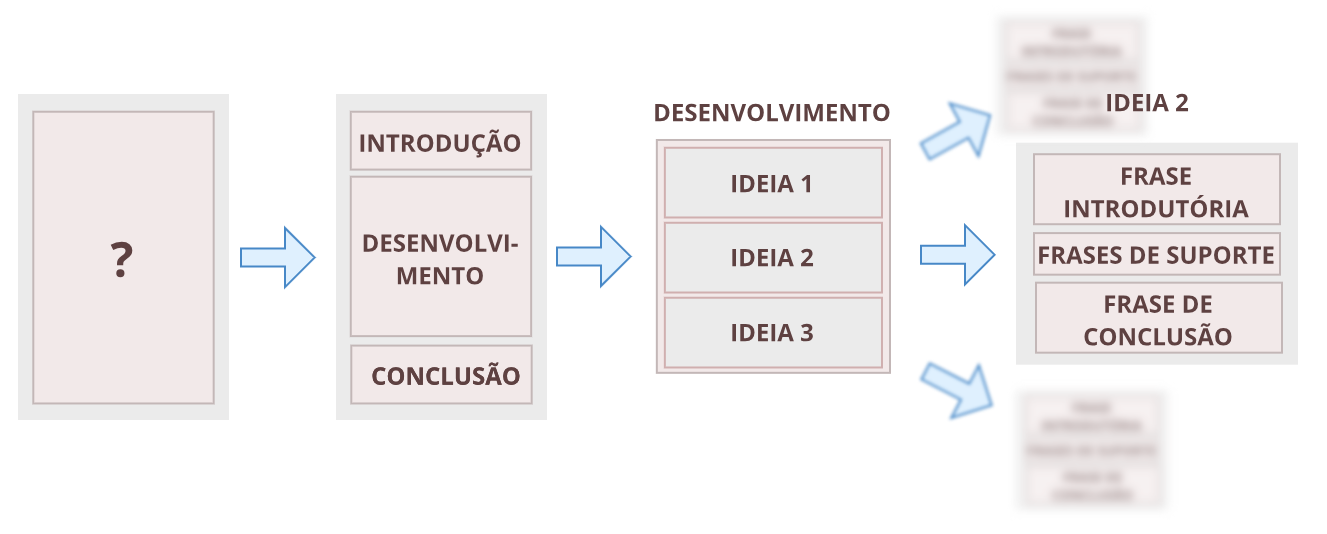
\includegraphics[width=1\linewidth]{figs/decomposition.png}    
            \end{center}
            
            \\ \hline
            
            \textbf{Reconhecimento de Padrões}: Identificar similaridades entre as partes de um problema para resolvê-las com eficiência \cite{bbc_learning_what_2015}. Na Ciência da Computação os padrões reduzem a complexidade por meio da generalização de soluções para aplicá-las em múltiplas situações \cite{k-12_computer_science_framework_k12_2016}. 
            &
            Um exemplo é reconhecer padrões em sequências de cores. A primeira vista são apenas círculos coloridos, mas é possível identificar o padrão sequencial de cores em cada linha. Outros exemplos são identificar rotas comuns entre casa e trabalho para organizar caronas, identificar o padrão de compras no mercado para dispor produtos, e também reconhecer sintomas similares de doenças entre pacientes.
            &
            \begin{center}
                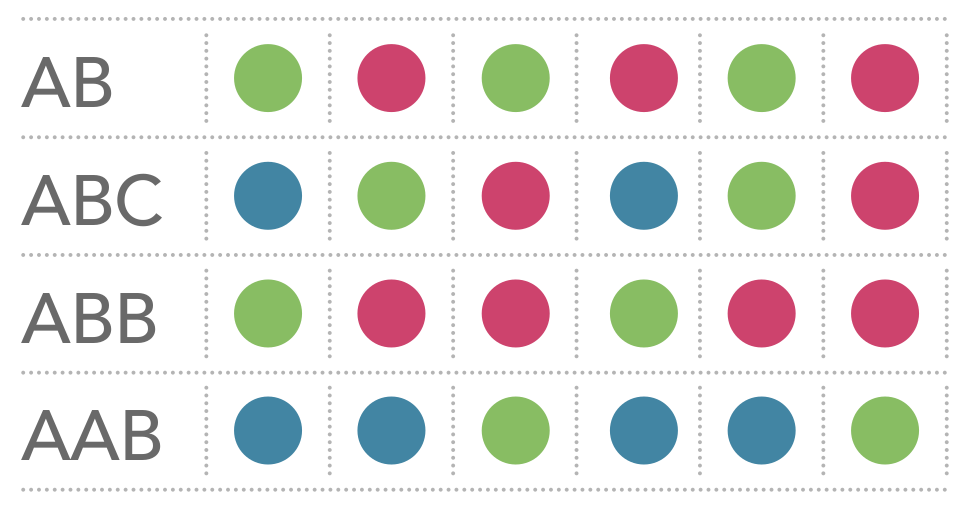
\includegraphics[width=1\linewidth]{figs/pattern_recognition.png}    
            \end{center}
            \\ \hline
            \textbf{Abstração}: Destacar detalhes importantes e ignorar detalhes desnecessários \cite{wing_computational_2008}. A abstração elimina os detalhes específicos, inúteis para resolver um problema, e cria uma ideia base da solução denominada modelo \cite{bbc_learning_what_2015}.
            &
            Durante o treinamento de cães farejadores para resgate de seres humanos, um conjunto de testes avalia os animais em quesitos como inteligência, concentração, agilidade e capacidade olfativa. Dados como raça, tamanho, cor ou peso não influenciam na capacidade do cão desempenhar a tarefa em questão. É preciso, portanto, detectar as características relevantes ao problema no universo de características do animal \cite{davidson_12_2018}.
            &
            \begin{center}
                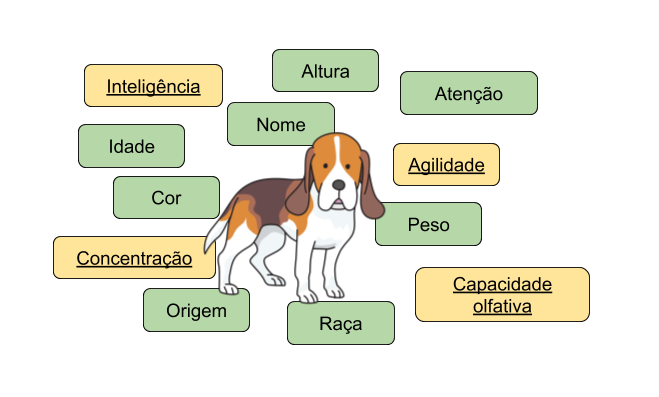
\includegraphics[width=1\linewidth]{figs/abstraction.png}    
            \end{center}
            
            \\ \hline
            \textbf{Algoritmos}: instruções que demonstram o passo a passo para resolver um problema. Esse conjunto de passos precisa ter um início, um fim, e uma sequência de instruções sem ambiguidade \cite{bbc_learning_what_2015}.
            
            &
            A representação desse conjunto de passos pode ocorrer por diferentes modos. Uma receita de bolo é um algoritmo, pois define o conjunto de passos para resolver o problema de criar um bolo. Neste caso a representação é textual, porém pode-se representar um algoritmo por fluxogramas, blocos, sequência de símbolos, etc.
            &
            \begin{center}
                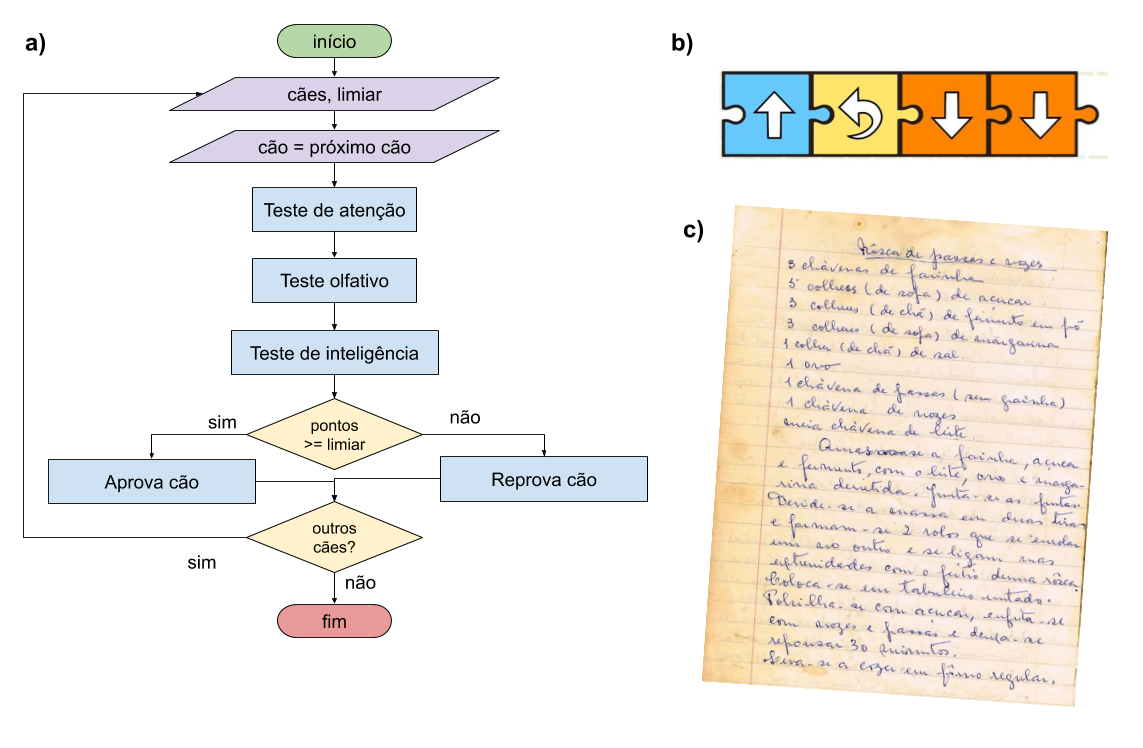
\includegraphics[width=1\linewidth]{figs/algoritmo.png}    
            \end{center}
            
            \\ \hline
            
        \end{tabular}
         
        \end{footnotesize}
    \end{center} 
    \end{quadro}
\end{landscape}

As definições de PC apresentadas estão relacionadas com resolução de problemas de modo geral, e não se restringem ao contexto da programação de algoritmos. Nessas definições, o conceito de depuração parece ter relevância secundária, sendo pouco citado. Uma possível causa é o fato da depuração estar "embutida" na prática de programar algoritmos, e não ser percebida como uma habilidade útil no dia a dia. \citeonline{mccauley_debugging_2008} comenta que até mesmo no campo da programação a depuração é negligenciada, afirmando que o livro de Barnes e Kölling (2002) é um dos poucos a dedicar um capítulo completo sobre depuração. A próxima seção busca esclarecer este conceito.

\subsection{Depuração}

A depuração é um conceito que foi particularmente discutido por pesquisadores e educadores nas décadas de 1970 \cite{mccauley_debugging_2008} e 1980 \cite{sipitakiat_robo-blocks_2012}. Mesmo já sendo praticada por programadores profissionais, foi o surgimento da linguagem Logo neste período que desencadeou estudos envolvendo depuração por crianças.  A recente popularização do PC e o aumento do contato de crianças com algoritmos tem levado pesquisadores a discutirem o papel da depuração no contexto educacional.

A atividade de depurar está ligada ao desejo de corrigir partes de algoritmos que impedem a execução correta de um programa. No contexto educacional este desejo cria uma situação propícia ao exercício de um conjunto maior de habilidades, como trabalho em equipe, comunicação e persistência \cite{spisipitakiat_robo-blocks_2012}. Portanto, pode ser vista como uma atividade de resolver problemas, que envolve observar, comunicar e refletir. A depuração, bem como a ação de ler e acompanhar a execução passo a passo de programas existentes são consideradas essenciais para aprender programação \cite{mccauley_debugging_2008}, e por consequência contribuir para o desenvolvimento do \ac{PC}.

Entretanto, \citeonline{liu_understanding_2017} observam que a depuração é um componente do PC negligenciado principalmente nos níveis iniciais de ensino. Os avanços tecnológicos e o entusiasmo com a temática do PC tem levado estudantes iniciarem o aprendizado de programação mais jovens. Ainda assim, afirma que poucos ambientes de programação são projetados com foco em funcionalidades de depuração no nível da Educação Básica, e a maior parte das pesquisas sobre o tema ocorrem com estudantes em nível universitário. 

\citeonline{brennan_new_2012} abordam a depuração em um framework de PC utilizado no contexto do ScratchJr. O framework tem três dimensões: conceitos, práticas e perspectivas. Os conceitos remetem aos conhecimentos utilizados e aprendidos durante a programação, como paralelismo, laços de repetição e dados. As práticas envolvem a aplicação desses conceitos utilizando de desenvolvimento iterativo, mesclagem de códigos e depuração. Por fim, as perspectivas são formas de se utilizar a tecnologia: como meio de expressão, conexão, e questionamento/mudança da realidade. Usando esse framework \citeonline{lye_review_2014} revisaram a literatura em busca de trabalhos sobre PC. Eles observam que 85\% dos artigos analisaram os aprendizados de PC relacionados a conceitos, e apenas 22\% analisaram as práticas. Argumentam que por isso seria necessário mais trabalhos ligados à praticas computacionais como a depuração.

\citeonline{wong_computational_2018} relacionam pensamento algoritmo e depuração como duas sub-habilidades do PC. O pensamento algorítmico seria a capacidade de formular sequências de passos para solucionar um problema independente de computador. A depuração seria aplicada depois do pensamento algorítmico, ao traduzir o algoritmo para um programa de computador e solucionar problemas no código do programa se este não gerar o resultado desejado. Papert, por outro lado, afirma que a depuração independe do computador, pois "estratégias de depuração foram desenvolvidas por estudantes de sucesso muito antes da existência dos computadores" \cite[p.23]{papert_mindstorms:_1980}. Seria, então, mais um processo mental do que o uso de ferramentas computacionais.

\citeonline{carver_assessing_1986} decompõem o processo da depuração em quatro etapas: (i) avaliar do programa, (ii) identificar o \bug, (iii) localizar o \bug, (iv) e corrigir o \bug. Em uma atividade com BPs, por exemplo (ver \autoref{fig_ex_carver_klar}), a criança executa o algoritmo e verifica se alcançou o resultado esperado. Caso contrário, precisa identificar o erro, por exemplo, se o brinquedo está no local errado, se virou para o lado errado, etc. Ainda na identificação, constrói hipóteses causas do problema. Faltou adicionar um comando de giro? O comando de giro está errado? A terceira etapa passa a ter contato com o código, onde a criança identifica qual peça pode ser o \bug. Por fim, na última etapa a criança modifica o programa, adicionando ou removendo a peça apontada na etapa 3 e o ciclo recomeça com uma nova execução.

\begin{figure}[!htpb]
  \centering
  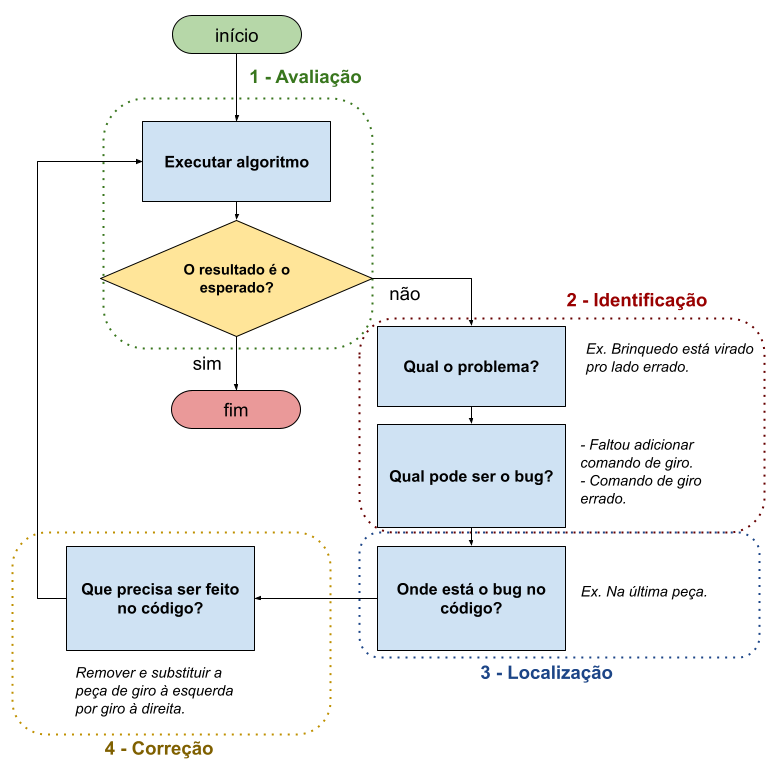
\includegraphics[width=.8\linewidth,fbox]{figs/ex_depuracao_carver_klar.png}
  \caption{Processo de depuração proposto por \citeonline{carver_assessing_1986} no contexto de um BP. }
  \sourceauthor
  \label{fig_ex_carver_klar}
\end{figure}

Seguindo esse modelo, \citeonline{carver_assessing_1986} avaliaram o aprendizado de depuração por crianças entre 7 e 8 anos. As crianças trabalharam em pares durante 22 horas de curso sobre a linguagem Logo. Os pesquisadores aplicaram 3 testes, sendo dois em dupla e um individual. Os testes avaliaram habilidade de depuração, interpretação de código, escrita de código e uso do ambiente Logo. Os resultados indicaram que as crianças depuraram somente quando lhes era solicitado, e que a estratégia utilizada para encontrar erros foi procurar linha por linha, sem uma estratégia eficiente. Os pesquisadores também perceberam que as crianças preferiram apagar o programa em vez de depurar. Por fim, concluem que depurar é uma atividade complexa, pouco ensinada, e que exige memória de trabalho para observar o programa criado e os problemas existentes. Além disso, menciona que o fato do erro ser punido pelo sistema educacional leva a criança a tentar eliminá-lo (apagar todo o programa) em vez de resolvê-lo.

\subsection{Depuração e visibilidade}
Em uma revisão sistemática, \citeonline{mccauley_debugging_2008} apresenta modelos de depuração definidos Vessey (1985) e Katz e Anderson (1987). Vessey (1985) define depuração em cinco passos: (i) determinar o problema comparando o resultado errado e o correto; (ii) \textit{obter familiaridade com a estrutura do programa}; (iii) explorar a execução do programa; (iv) levantar hipóteses para a causa do erro; e (v) reparar o erro. Katz e Anderson (1987) definem quatro passos: (i) entender o sistema, (ii) testar o sistema, (iii) \textit{localizar o erro}, e (iv) reparar o erro.

\begin{figure}[!htpb]
  \centering
  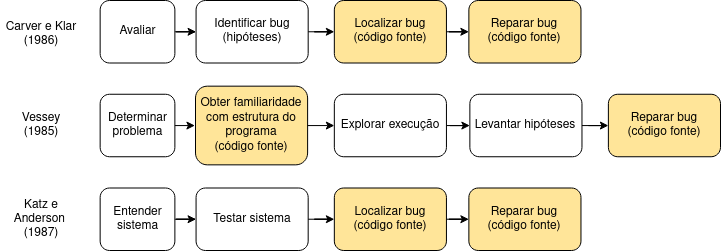
\includegraphics[width=.9\linewidth,fbox]{figs/debug_models.png}
  \caption{Modelos de depuração.}
  \sourceauthor
  \label{fig_debug_models}
\end{figure}

Estes modelos tem em comum um passo de observar a estrutura do algoritmo para localizar o erro (destacados na \autoref{fig_debug_models}). A localização do erro presume que um código fonte possa ser visto e analisado. Essa necessidade está ligada ao que \citeonline{norman_design_1988} apresenta como um dos princípios mais importantes do design: a visibilidade. Esse princípio permite o “mapeamento entre as ações pretendidas e as ações concretas” \cite{norman_design_1988}. Para isso, as ações possíveis de se realizar com uma interface devem estar visíveis e seus efeitos devem ser óbvios e imediatos.

A falta de visibilidade em interfaces de programação prejudica a depuração, que se revela em ferramentas projetadas para crianças. A Bee-Bot, por exemplo, é um brinquedo programado por botões de direção e tem um botão de limpeza de memória, que apaga os comandos do brinquedo. A falta de visibilidade se dá na ausência de um \textit{display} que mostre os comandos presentes na memória do brinquedo. Por não ver os comandos que estão programados, muitas vezes as crianças esquecem de limpar a memória do brinquedo e então pensam estar criando um novo programa \cite{raabe_brinquedos_2015}. A falta de visibilidade as impede de perceber que na verdade os comandos inseridos anteriormente ainda estão presentes, e os novos comandos estão sendo adicionados no final da sequência, criando um programa cada vez maior.

\citeonline{norman_design_1988} comenta que a visibilidade está ligada à formação de um modelo mental, por parte do usuário, de como determinado dispositivo funciona. Se os controles não estão claros e o dispositivo se comporta de maneira inesperada, o cérebro humano tenta encontrar uma explicação para tal comportamento. No caso da Bee-Bot, ao ver o brinquedo executar movimentos diferentes dos últimos comandos programados, as crianças tendem a entender que o brinquedo está tomando suas próprias decisões. Estão, portanto, formando um modelo mental inadequado quanto ao funcionamento do dispositivo computacional, ao não compreenderem que ele está executando uma sequência de passos pré-programados. 

Uma solução para o problema de falta de visibilidade em interfaces de programação pode estar na programação em blocos (\autoref{sec_prog_blocos}). \citeonline{wong_computational_2018} atribuem a melhoria na habilidade de depuração de crianças do 5º ano do Ensino Fundamental às "características de visualização da programação em blocos, pois os efeitos do programa podem ser vistos diretamente". \citeonline{bers_coding_2019} falam sobre as vantagens de visualização das interfaces de programação em blocos, neste caso blocos tangíveis:

\begin{citacao}
As crianças podem ver o que não funciona e podem ajudar a consertar. [...] A visibilidade adicional do código pode chamar a atenção para propriedades e conceitos anteriormente negligenciados, como elegância, a importância da depuração e teste para casos extremos e outras situações incomuns. Em outras palavras, o código tem o potencial de se tornar um objeto de conversa e atenção de uma forma que não poderia ser antes. \cite[p.14, tradução nossa]{bers_coding_2019}
\end{citacao}

Além de promover a visibilidade, a programação em blocos evita problemas de interação presentes em outros tipos de interface, como a programação textual.
Esta, apesar de também mostrar os comandos, não é acessível para crianças devido a erros de sintaxe e à necessidade de lembrar o que é preciso digitar. Os blocos, por outro lado, estão sempre disponíveis, geralmente agrupados por similaridade, de modo que não seja necessário lembrar sequências de caracteres para digitar num teclado. Além disso, o formato dos encaixes sugere como relacionar os blocos de modo coerente. 

A visibilidade da programação em blocos também favorece a interação social, tornando o código um objeto de conversa. O mesmo ocorre com a depuração, que é uma atividade estabelecida socialmente por meio de falas, apontamentos e olhares, e neste sentido os artefatos tem papel central \cite{heikkila_debugging_2018}. Esta ligação entre blocos e depuração favorece o princípio da linguagem Logo, de permitir depurar o que se passa na mente da criança \cite{solomon_history_2020}. Por meio de artefatos compartilhados socialmente, um adulto pode entender melhor o algoritmo que a criança tenta expressar. Assim, consegue auxiliá-la a desenvolver seu modelo mental de como construir um algoritmo para produzir um resultado desejado.

\section{Interfaces de Programação para Crianças}
\label{section_interfaces}

Aprender algoritmos parece ser uma tarefa difícil, mesmo para adultos. Analisando cursos de graduação em Computação de universidades dos Estados Unidos, Israel, Polônia e Austrália, \citeonline{mccracken_multi-national_2001} concluíram que os estudantes não possuíam as habilidades de programação esperada pelos professores, indicando dificuldade no aprendizado de algoritmos. \citeonline{hoed_alise_2016} cita a reprovação na disciplina de Algoritmos entre as causas de evasão em cursos de Computação. 

Felizmente, pesquisas sugerem que crianças podem aprender noções de algoritmos. \citeonline{sheehan_parent-child_2019}, observaram 31 crianças de 4.5 a 5 anos de idade, durante a interação com um aplicativo de programação. Os autores concluem que as crianças conseguiram produzir e compreender algoritmos básicos para definir o comportamento de um personagem. Em outro estudo, com 53 crianças de 4 a 6 anos, \citeonline{bers_computational_2014} identificam que 75\% das mesmas selecionaram e sequenciaram corretamente as instruções ao programar um veículo robótico. 

Os benefícios de aprender algoritmos transcendem os campos estritamente tecnológicos. Conforme lembram \citeonline{ciftci_effect_2020}, os algoritmos possuem conceitos que se intersectam com os da matemática, como variáveis, repetições e condicionais. Esses autores também afirmam que programar pode auxiliar estudantes analisarem seu modo de raciocínio, reorganizar tarefas seguindo um processo de resolução de problemas e desenvolver habilidades não-verbais. Em experimento, os autores verificaram um aumento significativo dessas habilidades em crianças de 4 a 5 anos que participaram de um curso de programação durante 8 semanas.

Para \citeonline{papert_mindstorms:_1980}, 

\begin{citacao}
Quando a criança aprende a programar, o processo de aprendizado é transformado. Ele se torna mais ativo e autodirigido. Em particular, o conhecimento é adquirido para um propósito pessoal reconhecido. A criança faz algo com ele. O novo conhecimento é uma fonte de poder e é experimentado como tal desde o momento em que começa a tomar forma na mente da criança \cite[p.21, tradução nossa]{papert_exploration_1996}.
\end{citacao}

Uma das primeiras experiências envolvendo crianças e programação é atribuída a Papert e Cynthia Solomon em 1968. Ambos foram até uma escola de um subúrbio de Boston ensinar programação para jovens. O computador que executou os programas estava em um laboratório a alguns quilômetros de distância. Por esse motivo, as crianças interagiram usando terminais, nos quais digitaram comandos na linguagem LOGO. 

Conforme novas versões da linguagem eram desenvolvidas, pesquisadores iam até as escolas para ensinar e observar o uso da linguagem em sala de aula \cite{bers_coding_2018}. Solomon destaca o papel da participação das crianças durante o desenvolvimento da linguagem, dando \textit{feedback} e influenciando diversas questões de design:

\begin{citacao}
O trabalho iniciou o que se tornou uma linguagem poderosa, flexível e usável para crianças e destacou a facilidade com que os aprendizes adquiriam expertise sobre a ferramenta. O trabalho é também um importante exemplo de envolvimento das crianças no design de uma nova tecnologia e de como a tecnologia pode se beneficiar da expertise e do \textit{feedback} das crianças. Cada vez que Seymour e eu trabalhamos com as crianças, LOGO foi radicalmente redesenhada incorporando o seu \textit{feedback}.
\end{citacao}

A linguagem LOGO inicialmente possibilitava manipular palavras, e deste modo as crianças construíam poemas e geradores de frases. Papert, um matemático, percebeu a necessidade transcender o campo das palavras e de permitir às crianças brincarem com formas, ângulos e desenhos. Dessa percepção nasceu a ideia de uma tartaruga capaz de se mover e desenhar figuras geométricas. Essa tartaruga foi instanciada primeiro virtualmente, mas depois tomou formas físicas e originando os primeiros brinquedos programáveis.

\subsection{Brinquedos Programáveis}
\label{brinquedos_programaveis}
Brinquedos programáveis são robôs cuja função é possibilitar a crianças o contato com conceitos matemáticos e algoritmos. O que os diferencia das outras ferramentas de programação é a aparência lúdica, que reflete o imaginário do público infantil \cite{raabe_rope_2017}. Pesquisas mencionam que os brinquedos programáveis podem promover habilidades relacionadas do \ac{PC} \cite{repiso_robotics_2019, bers_coding_2018, pugnali_impact_2017,  bers_computational_2014}, como pensamento algorítmico, reconhecimento de padrões, abstração e decomposição.

A interface intuitiva é o que permite que crianças possam programar esses brinquedos. A busca por interfaces intuitivas ocorre desde a linguagem LOGO, e com o desenvolvimento das tecnologias de hardware a diversas alternativas de interação tem surgido nos últimos anos \cite{catlin_edurobots_2018}. Por isso pesquisas tem buscado classificar essas interfaces.

\citeonline{hamilton_emerging_2020} apresentam 30 brinquedos e os classificam segundo suas características físicas em seis categorias: (i) jogos de tabuleiro ou livros; (ii) eletrônicos não robóticos; (iii) robôs controlados por tela; (iv) robôs operados por botões; (v) robôs com interface tangível; e (vi) híbridos \autoref{hamilton}. 

\begin{figure}[!htpb]
  \centering
  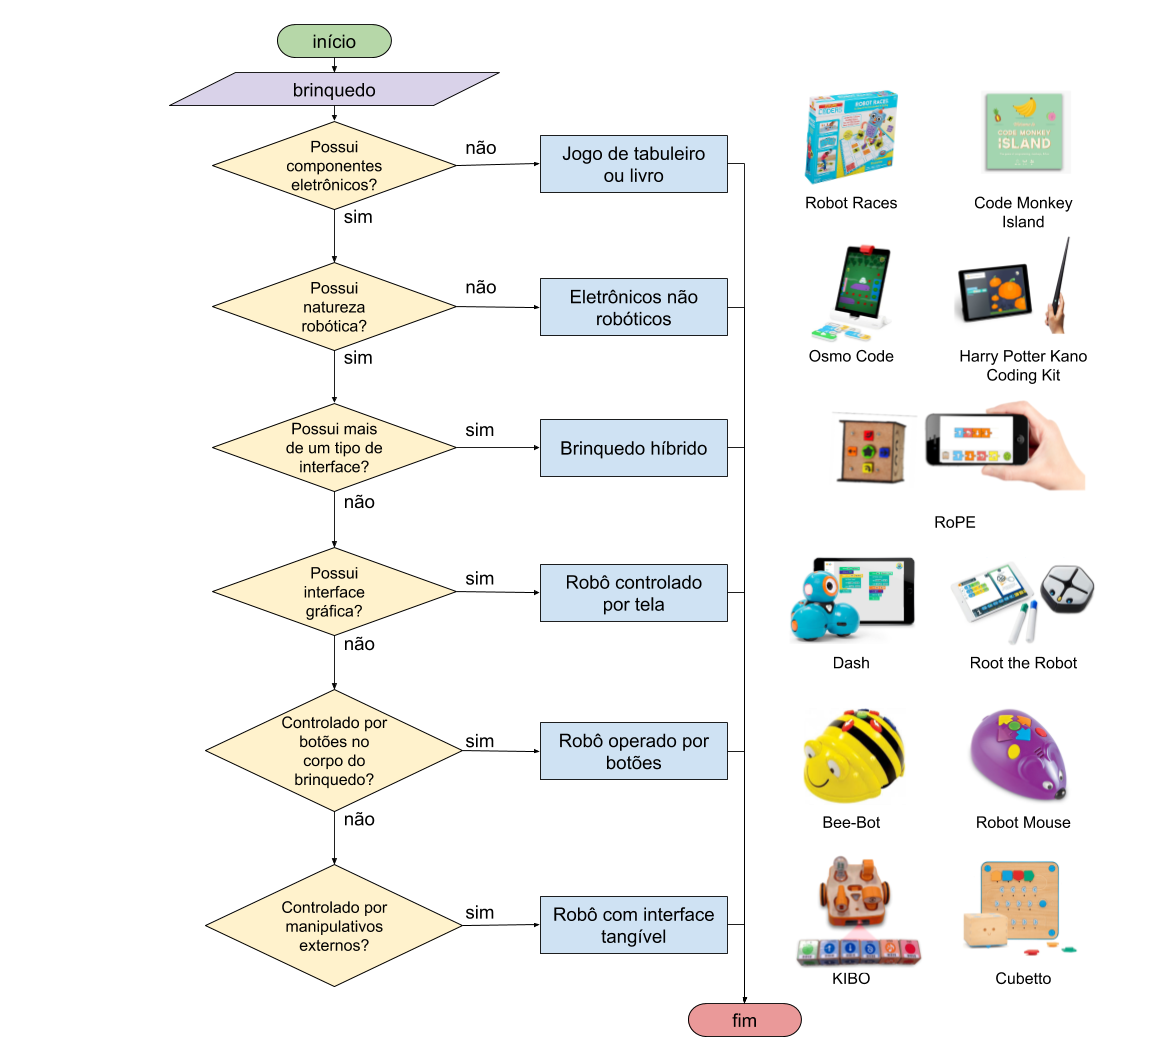
\includegraphics[width=.9\linewidth,fbox]{figs/hamilton_classification.png}
  \caption{Classificação de brinquedos programáveis por características físicas.}
  \source{ Adaptado de \citeonline{hamilton_emerging_2020}.}
  \label{hamilton}
\end{figure}

Em outra revisão, \citeonline{yu_review_2019} também analisam um conjunto de 30 brinquedos programáveis e kits de robótica focados em crianças de até 7 anos. A análise ocorre sob as perspectivas de design, \acl{PC}, expressividade e suporte a domínios\footnote{
A expressividade corresponde à variedade de atividades possibilitadas pelo kit, e o suporte a domínios se refere ao conjunto de assuntos/conteúdos passíveis de serem apresentados no contexto dessas atividades.
}.

Quanto ao design, \citeonline{yu_review_2019} distinguem três categorias de kits: físicos, virtuais e híbridos. As três categorias têm o comum a utilização de blocos de código relacionados a movimentos, com cada bloco tendo uma cor diferente para auxiliar na distinção dos diferentes
comandos. Esses blocos comumente tem o formato de peças de quebra-cabeça. Os kits físicos, como KIBO e Cubetto, possuem todos os componentes tangíveis, geralmente incluindo um robô com rodas, um conjunto de blocos de código e materiais de suporte como mapas, livros e materiais de personalização. Alguns robôs são controlados por botões, mas a maioria tem blocos de códigos separados.

Os kits virtuais são aqueles que não possuem parte tangível. Exemplos são aplicativos de \textit{smartfone} e jogos de computador, que possibilitam construir cenas, programar personagens e resolver problemas ao arrastar e soltar blocos de código virtuais. O Scratch e o ScrachJr são exemplos de aplicativos que permitem construir cenas e programar personagens. Essa categoria remete às primeiras experiências de Papert durante o desenvolvimento da linguagem logo, quando permitia definir o comportamento da tartaruga virtual. A diferença é que as ferramentas atuais
priorizam o uso de linguagens de blocos para evitar erros de sintaxe.

A terceira categoria são os kits híbridos, onde há união de partes tangíveis e virtuais. \citeonline{yu_review_2019} destacam que há dois tipos de kits híbridos: aqueles com blocos físicos que controlam personagens virtuais (brinquedos da empresa Osmo, por exemplo\footnote{\url{https://www.playosmo.com/en/coding/}}), e aqueles que possuem blocos virtuais para controlar personagens físicos.

Quanto ao \acl{PC}, \citeonline{yu_review_2019} relacionam atividades possibilitadas pelos BPs e kits capazes de promover os conceitos e práticas ligadas ao \ac{PC} definidas por \citeonline{brennan_new_2012}. Os autores identificam que as atividades com BPs podem abordar todos os conceitos e práticas do \ac{PC}. Há poucos kits, porém, que suportam as práticas de reutilização/combinação e abstração/modularização.

\begin{quadro}[!htbp]
 \caption{Como brinquedos programáveis e kits promovem conceitos e práticas computacionais.}
 \label{quadro_brinquedos_praticas} 
 \begin{center}
 \begin{footnotesize} 
\begin{tabular}{|p{3cm}|p{12cm}|}
\hline
\multicolumn{2}{|c|}{\textbf{Conceitos}} \\ \hline

    Sequenciamento & Criar uma sequência de código para programar o movimento ou outros efeitos em robôs físicos ou virtuais. \\ \hline
    
    Repetições & Encapsular uma sequência de comandos em blocos de repetição para executar repetidas vezes. \\ \hline
    
    Eventos & Executar ações ao apertar botões específicos, ou programar efeitos durante interações entre brinquedos (por exemplo, Dash e Dot executam ações quando se aproximam um do outro). \\ \hline
    
    Paralelismo & Controlar o movimento de diversos robôs/sprites simultaneamente, ou programar efeitos simultâneos de movimento, luzes e sons. \\ \hline
    
    Condicionais & Programar ações dependentes de eventos disparados por sensores ou mapas. \\ \hline
    
    Operadores & Possibilitar realizar operações matemáticas simples. \\ \hline
    
    Dados & Ajustar parâmetros como distância do movimento, rotação, etc. \\ \hline

\multicolumn{2}{|c|}{\textbf{Práticas}} \\ \hline

    Desenvolvimento iterativo e incremental & Permitir erros e tentativas ilimitados. Constantemente revisar e adicionar novos blocos de código (ex. ScratchJr). \\ \hline
    
    Teste e depuração & Testar continuamente o código durante o desenvolvimento e depurar se algo não funciona. \\ \hline
    
    Reutilização e combinação & Construir projetos partindo de projetos anteriores (ex. Scratch). A maioria dos kits não suporta essa prática. \\ \hline
    
    Abstração e modularização & Construir blocos de código que podem ser chamados de outros locais (ex. Cubetto). Poucos kits suportam essa prática. \\ \hline

\end{tabular}
 
 \end{footnotesize}
 \end{center} 
 \source{Adaptado de \citeonline{yu_review_2019}.}
\end{quadro}

Quanto à expressividade, ou seja, as atividades que os brinquedos possibilitam, os autores citam três principais modalidades. A primeira corresponde a mover o brinquedo/kit por um caminho ou sobre um mapa para coletar objetos. A segunda modalidade é a contação de histórias: os brinquedos se movem sobre cenários, e as crianças podem criar histórias para os mesmos em conjunto com a família. Há também um terceiro tipo de atividade: decorar e personalizar a aparência do brinquedo.

Quanto ao suporte a domínios, \citeonline{yu_review_2019} mencionam o desenvolvimento de narrativas, conceitos matemáticos e conceitos de engenharia. O desenvolvimento de narrativas está ligado às atividades de contação de histórias. O Scratch, por exemplo, possibilita criar narrativas por meio da programação de personagens e definição de cenários. Conceitos matemáticos aparecem ao definir distâncias de movimentos, e operações aritméticas simples também estão presentes em alguns brinquedos. Os conceitos de engenharia são abordados em brinquedos onde é possível unir partes diversas e observar efeitos, como o caso do Cubelets\footnote{\url{https://www.modrobotics.com/\#whatr-cubelets}}, que permite à criança unir cubos de luminosidade, sensores e movimentos.

As classificações de \citeonline{hamilton_emerging_2020} e de \citeonline{yu_review_2019} se diferem quanto aos critérios utilizados. Enquanto \citeonline{hamilton_emerging_2020} não inclui em sua lista os kits robóticos e softwares exclusivamente gráficos, \citeonline{yu_review_2019} inclui ambos. Ambos os trabalhos, porém, tem foco o público infantil, e as análises das interfaces e dos conceitos promovidos são úteis para definir as características do brinquedo RoPE.

\subsubsection{RoPE - Robô Programável Educacional}
O RoPE é um brinquedo programável desenvolvido para crianças a partir de 3 anos, que busca estimular o \acl{PC} e a criatividade. Ele permite à criança inserir comandos que ele então executa em forma de movimentos sobre um tapete temático. A construção tem preocupações de design relacionadas às crianças e ao ambiente. Quanto às crianças, o tamanho dos botões leva em conta que a coordenação motora ainda está em desenvolvimento. Quanto ao ambiente, as cores dos botões facilitam a comunicação das professoras para indicarem um botão específico durante alguma explicação.

\begin{figure}[!htpb]
  \centering
  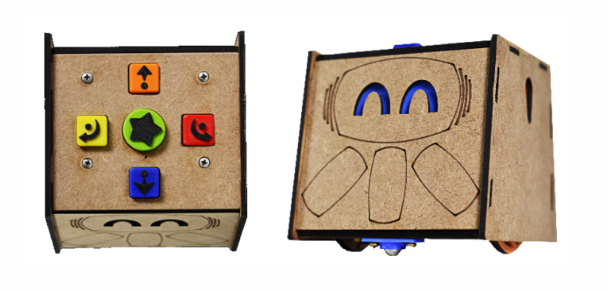
\includegraphics[width=.9\linewidth,fbox]{figs/rope_up_front.png}
  \caption{Visão superior e frontal do RoPE.}
  \source{Smartfun Brasil.}
  \label{rope}
\end{figure}
O RoPE pode ser operado de duas formas: botões na parte superior e um aplicativo de \textit{smartphone}. A primeira interface é formada por 5 botões que fazem parte do brinquedo. Seus comandos são (1) girar para esquerda 90 graus, (2) girar para direita 90 graus, (3) movimentar para frente (4) movimentar para trás, e (5) executar instruções da memória ou limpar memória. A execução de cada instrução provoca, além do movimento, a emissão de um som característico e uma luz da mesma cor do botão gerador da instrução, de forma a haver uma tríade cor-movimento-som. Um som de finalização indica quando o brinquedo executou todas as instruções \cite{raabe_rope_2017}.

A segunda interface é um aplicativo de celular que permite programar o RoPE a distância (\autoref{rope_app}). O programa aparece na tela em formato de peças de quebra-cabeça conectadas. A comunicação Bluetooth entre o brinquedo e o aplicativo possibilita manter as peças e as instruções da memória em sincronia. A reordenação das peças no aplicativo é replicada no brinquedo e o pressionamento de um botão do brinquedo é replicado nas peças na tela do celular. Considerando, então, a possibilidade de programar por meio de duas interfaces, as classificações de \citeonline{hamilton_emerging_2020} e \citeonline{yu_review_2019} posicionam o RoPE como um brinquedo híbrido.

\begin{figure}[!htpb]
  \centering
  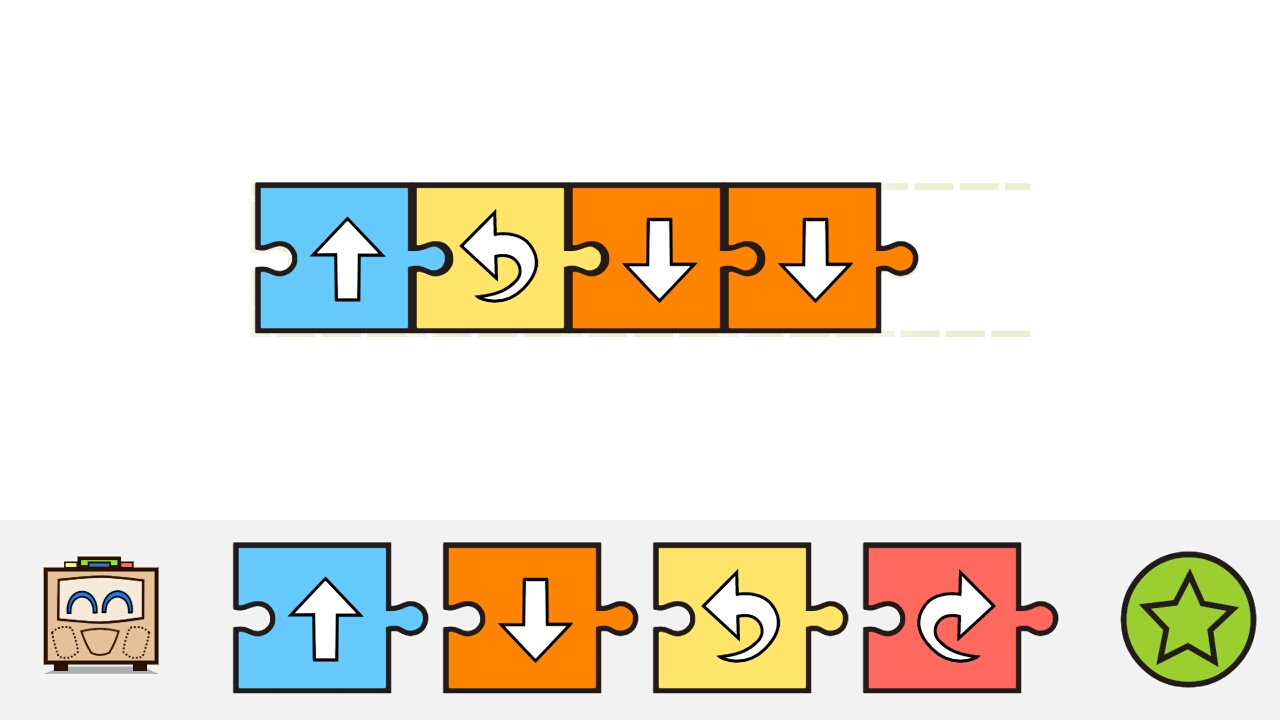
\includegraphics[width=.9\linewidth,fbox]{figs/app.jpg}
  \caption{Aplicativo para programar o RoPE.}
  \sourceauthor
  \label{rope_app}
\end{figure}

O \autoref{quadro_rope_pc} classifica o RoPE quanto aos aspectos do \acl{PC}. Os conceitos abordados pelo brinquedo são sequenciamento, eventos e dados. O brinquedo aborda diretamente apenas sequenciamento e eventos, porém as professoras podem abordar o conceito de dados durante o uso do brinquedo, ao definir distâncias e posições a serem alcançadas. O brinquedo não abrange todas as práticas e conceitos pois o público-alvo são crianças da Educação Infantil e é preciso manter um design simplificado.

\begin{quadro}[!htbp]
 \caption{Conceitos e práticas computacionais e sua promoção pelo brinquedo RoPE.}
 \label{quadro_rope_pc} 
 \begin{center}
 \begin{footnotesize} 
\begin{tabular}{|p{5cm}|p{10cm}|}
\hline
\multicolumn{2}{|c|}{\textbf{Conceitos}} \\ \hline
    
    Sequenciamento & Criar uma sequência de comandos para guiar o movimento do RoPE sobre um mapa. \\ \hline
    
    Repetições & \notcovered \\ \hline
    
    Eventos & O evento de clicar na estrela inicia a execução dos comandos inseridos previamente. \\ \hline
    
    Paralelismo & \notcovered \\ \hline
    
    Condicionais & \notcovered \\ \hline
    
    Operadores & \notcovered \\ \hline
    
    Dados & Estimar o número de passos para alcançar uma posição no mapa. \\ \hline

\multicolumn{2}{|c|}{\textbf{Práticas}} \\ \hline

    Desenvolvimento iterativo e incremental & Não abordado diretamente, pois as instruções são apagadas do brinquedo ao final de cada execução. \\ \hline
    
    Teste e depuração & Testar continuamente o código durante o desenvolvimento e depurar se algo não funciona. \\ \hline
    
    Reutilização e combinação & \notcovered \\ \hline
    
    Abstração e modularização & \notcovered \\ \hline

\end{tabular}
 
 \end{footnotesize}
 \end{center} 
 \sourceauthor
\end{quadro}

Além de aspectos ligados ao PC, o RoPE suporta domínios multidisciplinares por meio de tapetes temáticos, nos quais as crianças tem contato com letras do alfabeto (\autoref{tapete_alfabeto}), temáticas dos ambientes rurais (\autoref{tapete_farm}) e urbanos (\autoref{tapete_city}). \citeonline{pinheiro_alise_2016} desenvolveu um software que permite à criança gerar seus próprios mapas e percebeu mais engajamento das crianças ao usarem seus próprios mapas. Esses tapetes também podem ser criados manualmente, como o tapete criado pelas crianças da \autoref{tapete_alfabeto}. Além de criar os próprios tapetes \citeonline{martins_desenvolvimento_2016} também menciona a possibilidade de customizar a carcaça do brinquedo. Então, apesar de a interface do brinquedo favorecer raciocínio matemático de estimar quantidades e movimentos, a customização e os tapetes possibilitam criar micromundos infinitos associados a qualquer temática.

\begin{figure}[!htbp]
    \centering
    \begin{subfigure}{.33\textwidth}
        \centering
        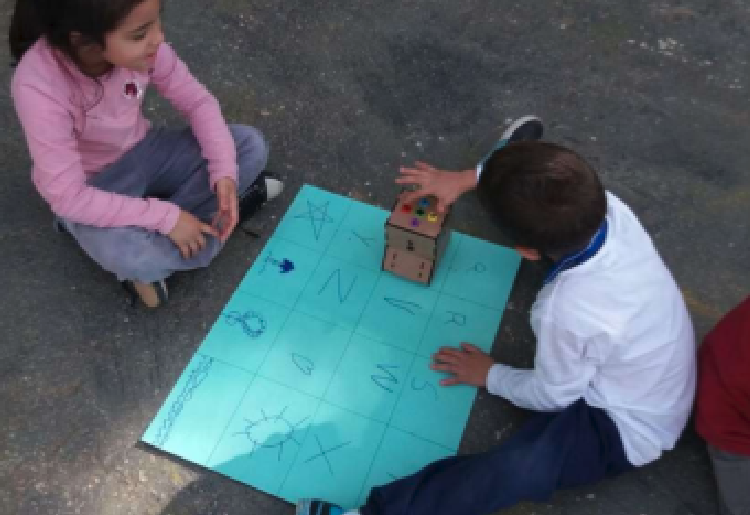
\includegraphics[width=.9\linewidth,fbox]{figs/tapete_alfabeto.png}
        \caption{Letras do alfabeto}
        \label{tapete_alfabeto}
    \end{subfigure}%
    \begin{subfigure}{.33\textwidth}
        \centering
        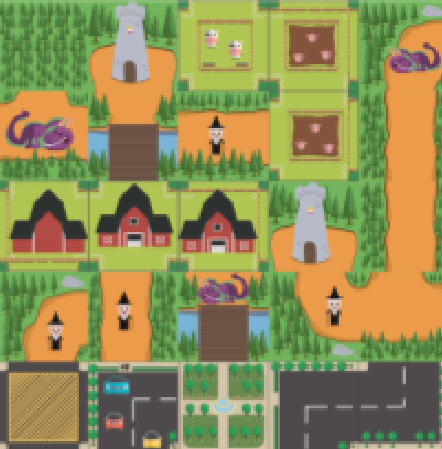
\includegraphics[width=.9\linewidth,fbox]{figs/tapete_farm.png}
        \caption{Ambiente rural}
        \label{tapete_farm}
    \end{subfigure}
    \begin{subfigure}{.33\textwidth}
        \centering
        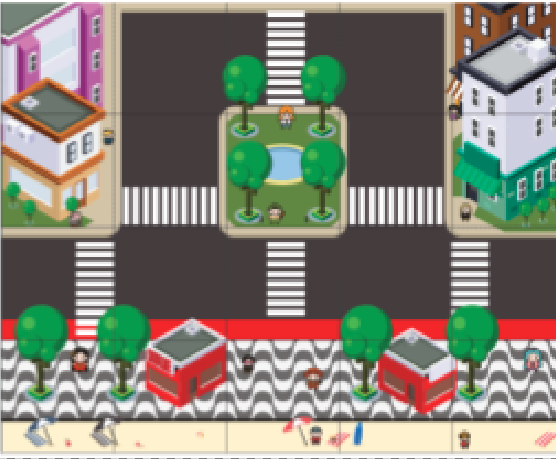
\includegraphics[width=.9\linewidth,fbox]{figs/tapete_city.png}
        \caption{Ambiente urbano}
        \label{tapete_city}
    \end{subfigure}
    \caption{Tapetes temáticos.}
    \sourceauthor
    \label{rope_mats}
\end{figure}

\subsection{Interfaces Tangíveis}
\label{fundamentacao_sub_interfaces_tangiveis}
Como abordado na \autoref{brinquedos_programaveis}, as interfaces tangíveis representam um dos tipos de interfaces utilizadas pelos brinquedos de programar. O conceito de interfaces tangíveis, entretanto, é amplo e tem fronteiras difusas \cite{falcao_design_2007}. A ideia inicial sobre tangibilidade é que apresenta formas físicas de interação, que permitem o contato da mão com objetos concretos. Essa forma de interação é considerada mais intuitiva e capaz de estimular colaboração e diversão (ZUCKERMAN; GAL-OZ, 2013). A tangibilidade dos blocos de encaixar como LEGO, por exemplo, leva crianças a permanecerem horas manipulando-os e testando possibilidades de construções. 

Mas somente a ideia de manipulação de objetos concretos não delimita o que são interfaces tangíveis. Como questionado por \citeonline[p.30]{falcao_design_2007}, dado que são manipulados diretamente, “teclados são TUIs?”. Neste sentido, diferentes taxionomias buscam organizar a definição de interfaces tangíveis \cite{fishkin_taxonomy_2004, fincher_tangible_2019}. \citeonline{fishkin_taxonomy_2004}, por exemplo, observa a sequência de ações do usuário durante uma interação. Em toda interação, primeiramente o usuário manipula uma interface e em seguida observa o resultado da manipulação. A taxonomia considera o quão distante estão os pontos de manipulação e o ponto de expressão do resultado. Esta distância é chamada de “incorporação”. Quanto mais próxima a manipulação está do resultado, maior a incorporação. Há quatro níveis de incorporação das interfaces tangíveis:

\begin{description}
    \item[Completa:] O ponto de manipulação é o mesmo que expressa o resultado. Um exemplo é o ábaco.
    \item[Próxima:] A expressão do resultado ocorre próxima do ponto de manipulação. Uma caneta é um exemplo.
    \item[Ambiental:] A expressão do resultado está "ao redor"\ do usuário. Um exemplo seria uma sala com projeção nas paredes.
    \item[Distante:] O ponto de manipulação e a expressão do resultado ficam em salas separadas, ou a metros de distância. O controle remoto é um exemplo.
\end{description}

\citeonline{fincher_tangible_2019} organizam as linguagens tangíveis de programação em três categorias:

\begin{description}
    \item[Linguagens de blocos inteligentes:] Blocos físicos com componentes eletrônicos internos estão nessa categoria. Eles são capazes de armazenar instruções e também executá-las.
    
    \item[Linguagens de demonstração:] Neste caso o usuário demonstra ao dispositivo o que deve ser executado e então ele reproduz. A demonstração pode ocorrer por meio de gestos, sons ou entradas digitais (botões).
    
    \item[Linguagens externamente compiladas:] São representações simbólicas do programa a que não possuem componentes eletrônicos. Algum agente externo, como uma câmera, capta os símbolos e transmite para um componente compilar o programa. Exemplos são blocos de madeira como utilizado pelo brinquedo KIBO.
\end{description}

Por fim, \citeonline{falcao_design_2007} respondem a própria pergunta: teclados e mouse não são TUIs pois não carregam em si um significado. Ao contrário, são dispositivos genéricos capazes de gerar significados variados. Por outro lado, o ábaco é uma interface tangível pois traz incorporado o significado numérico. Blocos de madeira, como usados pelo KIBO, é uma linguagem externamente compilada que traz em si o significado de um algoritmo.

\subsection{Programação em Blocos}
\label{sec_prog_blocos}
Programação em blocos tem se tornado a forma mais comum de iniciar o aprendizado de programação \cite{weintrop_block-based_2019}. Ferramentas como o Scratch, ScratchJr e o Code.org utilizam essa abordagem. \citeonline{bordini_computacao_2016}, em revisão sobre o \acl{PC} no Brasil, identificaram que mais de 40\% das iniciativas para ensino de programação adotou ambientes baseados em blocos para introduzir os primeiros conceitos. 

A programação em blocos se caracteriza por blocos semelhantes a peças de quebra-cabeça, que encaixados representam um algoritmo. As cores e o formato indicam quando e como cada bloco pode ser usado. O formato do encaixe, por exemplo, evita erros de sintaxe \cite{weintrop_block-based_2019}. Além disso, o usuário pode explorar os blocos disponíveis e isso tende a mitigar a necessidade de ler de documentações. 

Apesar de mitigar a necessidade de digitação, a programação em blocos não significa o fim da necessidade de leitura. Há blocos que contém texto, o que aumenta a complexidade para crianças em processo de alfabetização \cite{flannery_designing_2013}. Um exemplo é o Scratch (\autoref{scratch_blocks}).

Tendo em vista esta questão, o ScratchJr é um ambiente de programação desenvolvido para crianças, como alternativa ao Scratch. O Scratch é um ambiente de programação que utiliza texto em seus blocos e portanto não é indicado para crianças menores de 5 anos. O ScratchJr, por outro lado, tem ícones em seus blocos (\autoref{scratch_jr_blocks}).

\begin{figure}[!htbp]
    \centering
    \begin{subfigure}{.35\textwidth}
        \centering
        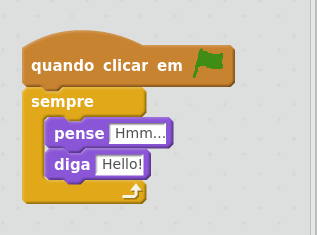
\includegraphics[width=.9\linewidth,fbox]{figs/scratch_blocos.png}
        \caption{Blocos do Scratch}
        \label{scratch_blocks}
    \end{subfigure}%
    \begin{subfigure}{.65\textwidth}
        \centering
        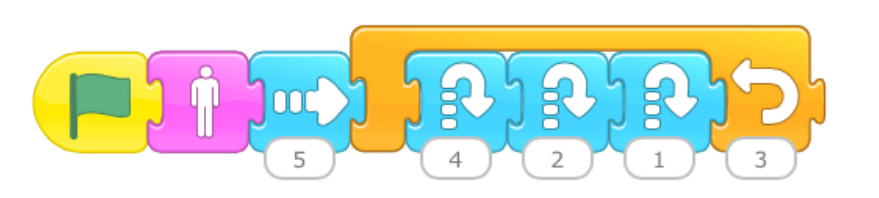
\includegraphics[width=.9\linewidth,fbox]{figs/scratch_jr.png}
        \caption{Blocos do ScratchJr}
        \label{scratch_jr_blocks}
    \end{subfigure}
    \caption{Blocos do Scratch e do ScratchJr.}
    \sourceauthor
    \label{scratch_scratch_jr_blocks}
\end{figure}

Além dos ambientes gráficos, a programação em blocos também existe em interfaces tangíveis. Os blocos gráficos mitigam a necessidade de digitação, porém ainda é dependem do mouse ou telas sensíveis ao toque para arrastar e soltar. Os blocos físicos eliminam essa necessidade, permitindo a manipulação direta e natural. O Osmo (\autoref{osmo_blocks}) é um exemplo de uso de blocos tangíveis de programação. Os blocos são identificados pela câmera de um tablet, e um personagem na tela executa os comandos programados. O Cubetto, já apresentado, utiliza blocos que são encaixados em um painel de madeira (\autoref{cubetto_blocks}).

\begin{figure}[!htbp]
    \centering
    \begin{subfigure}{.56\textwidth}
        \centering
        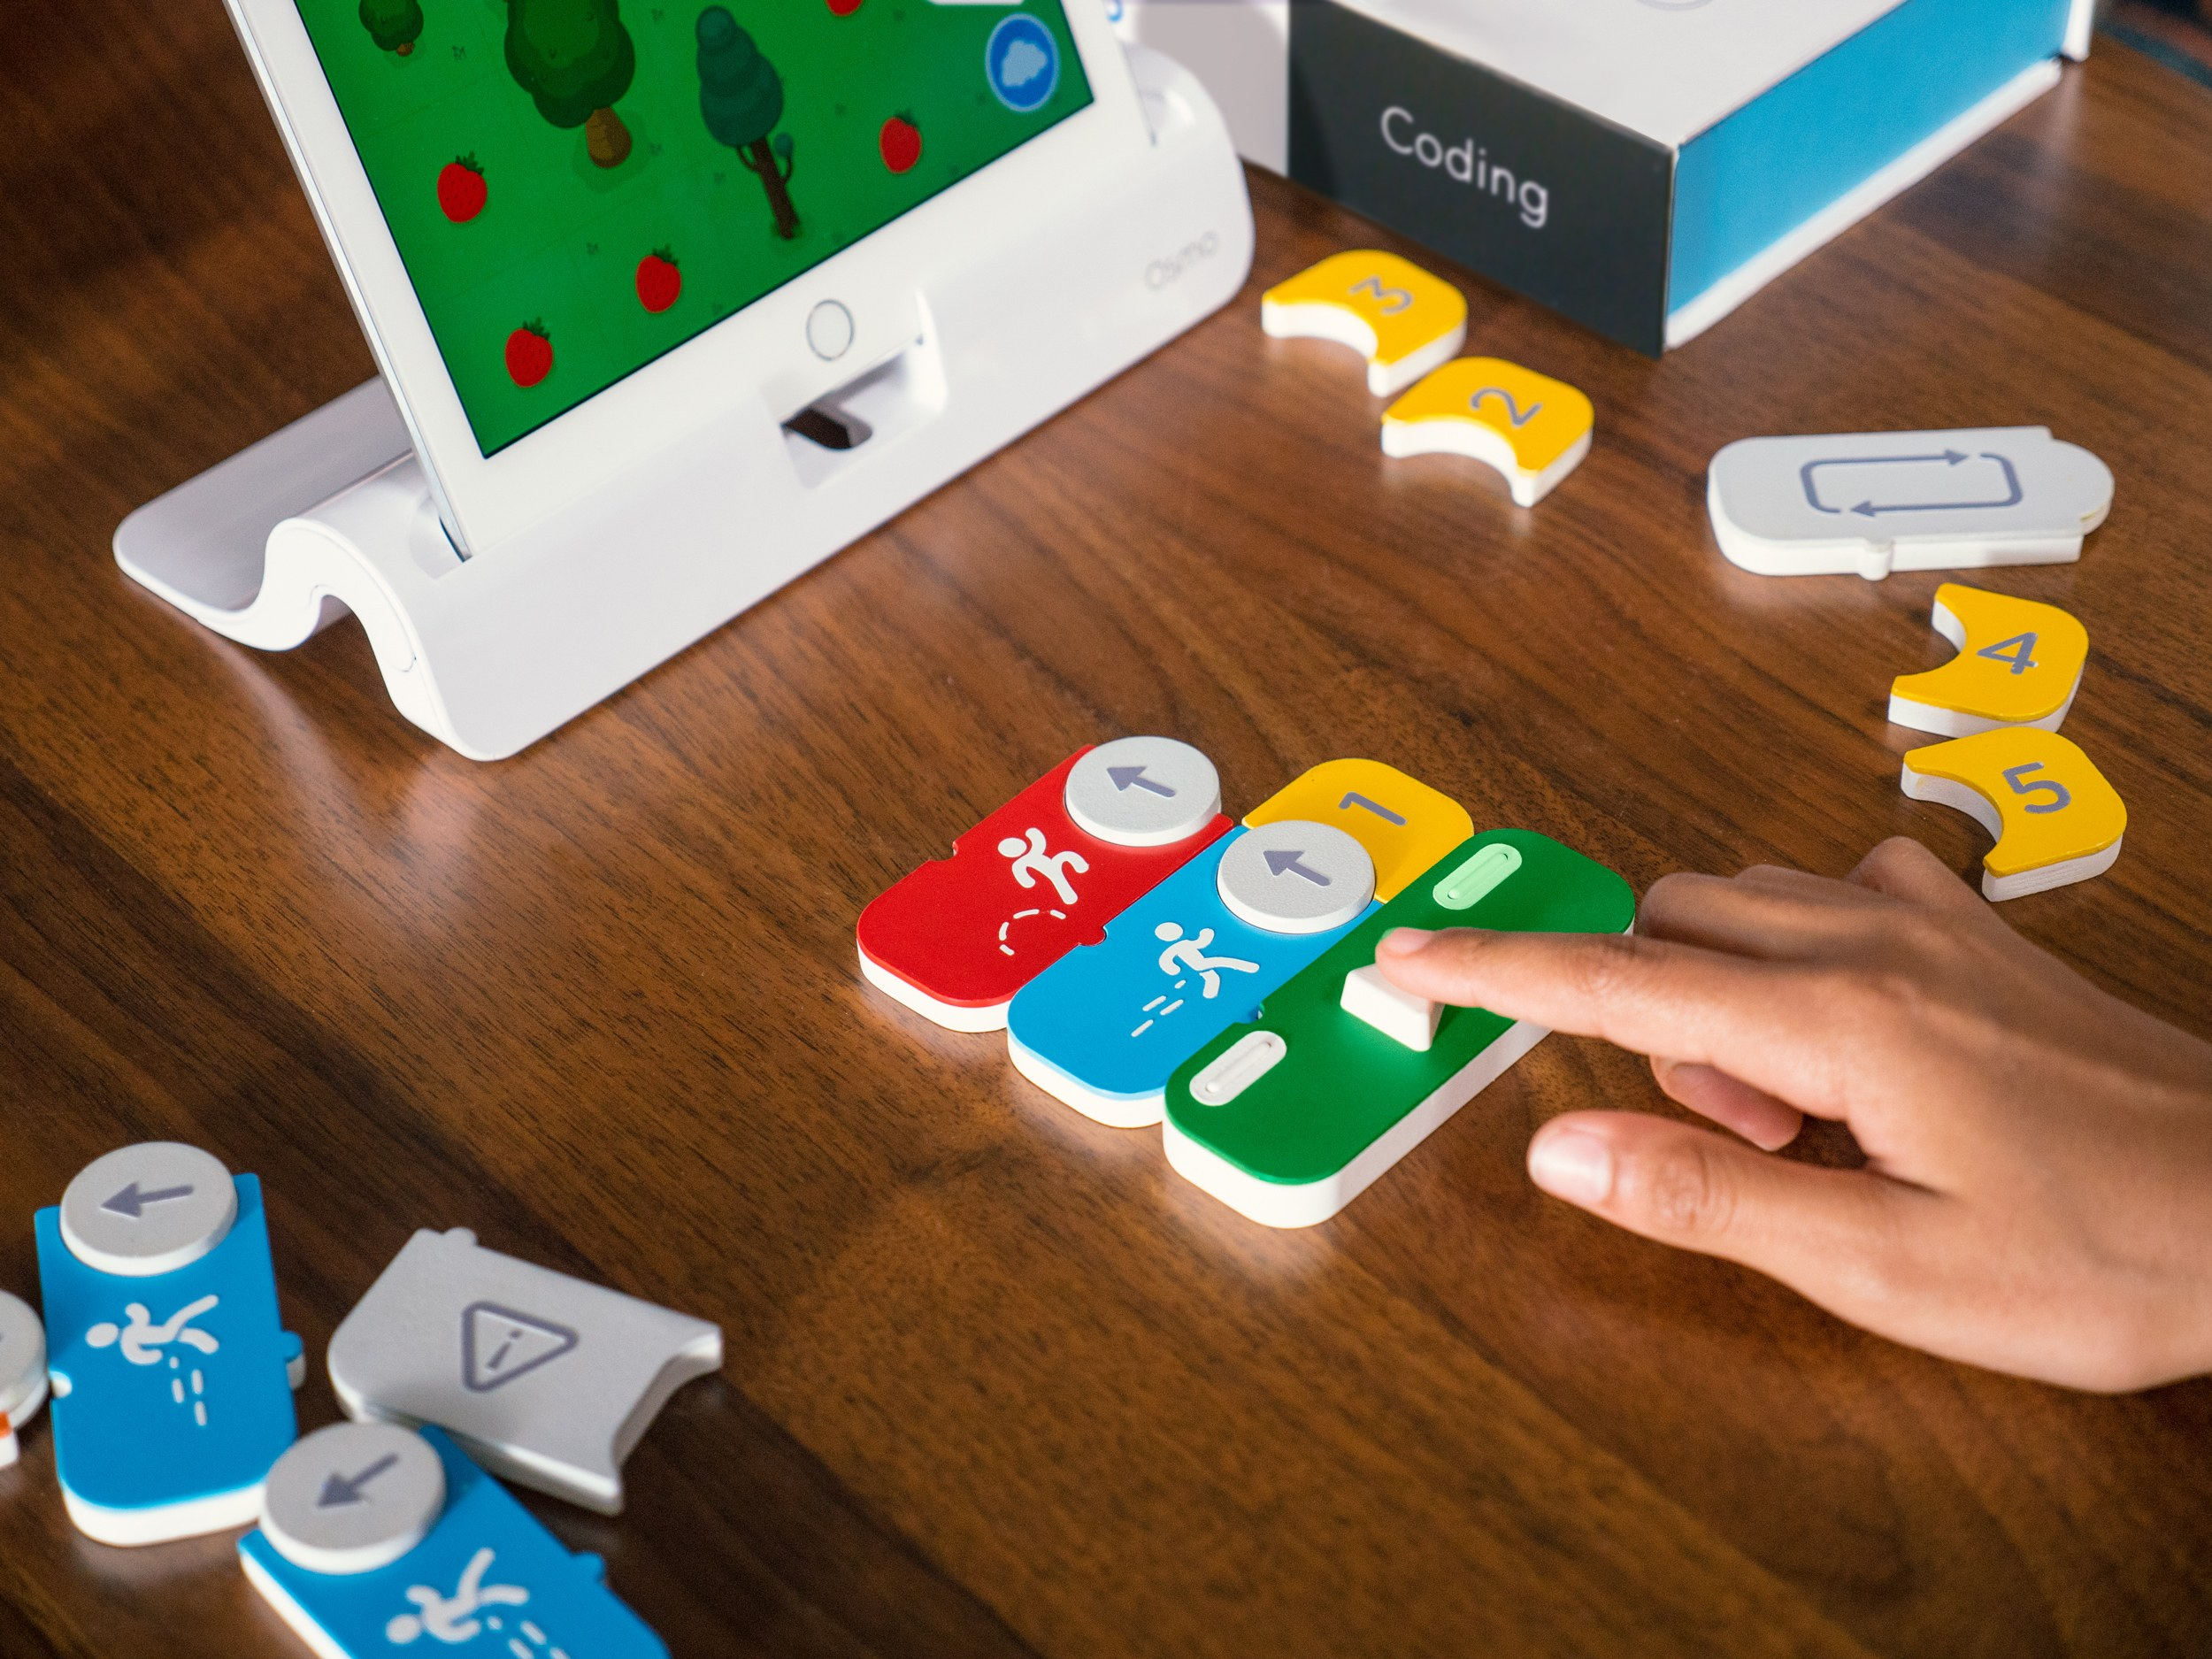
\includegraphics[width=.9\linewidth,fbox]{figs/osmo.jpg}
        \caption{Osmo}
        \label{osmo_blocks}
    \end{subfigure}%
    \begin{subfigure}{.43\textwidth}
        \centering
        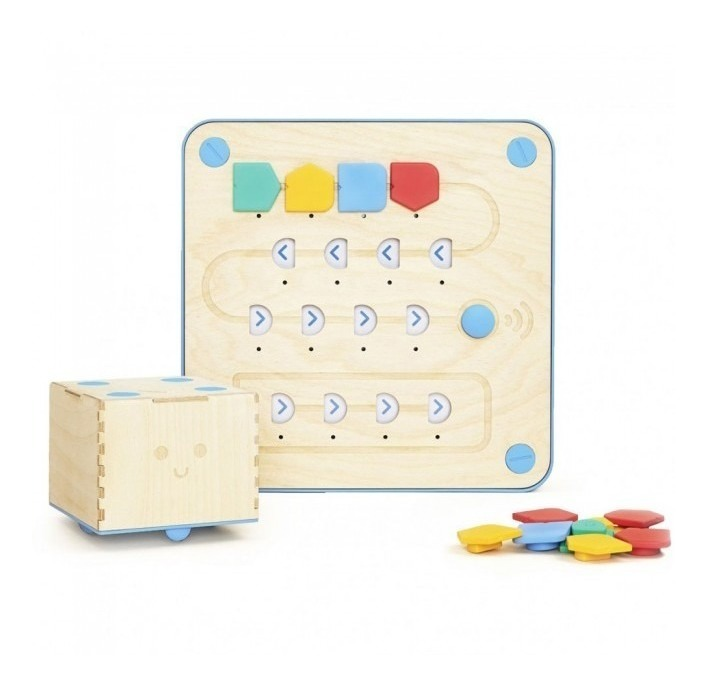
\includegraphics[width=.9\linewidth,fbox]{figs/cubetto.jpg}
        \caption{Cubetto}
        \label{cubetto_blocks}
    \end{subfigure}
    \caption{Blocos tangíveis.}
    \sourceauthor
    \label{tangible_blocks}
\end{figure}

Uma vantagem do painel do Cubetto é indicar, por meio de luzes, qual bloco está sendo executado em cada momento. Isso permite acompanhar a execução, o que é um processo de depuração. Possíveis desvantagens do painel são a limitação do número de encaixes disponíveis e a necessidade de um hardware específico.

\subsection{Marcas Fiduciais}
\label{sub_sec_fiduciais}
Interfaces tangíveis aplicam diferentes técnicas de captura de blocos físicos. O Cubetto depende de um hardware específico para identificar os blocos encaixados em um painel, e o Osmo utiliza visão computacional. Uma alternativa que pode facilitar a demarcação de objetos físicos na construção de interfaces tangíveis, e também na construção de aplicações de Realidade Aumentada (\autoref{sub_sec_fiduciais}), são as marcas fiduciais. 

Marcas fiduciais (\autoref{fiducial}) são padrões de figuras desenvolvidas com o objetivo de facilitar a identificação e localização de pontos de referências em imagens. Sistemas de marcas fiduciais são compostos por modelos de marcas e um algoritmo capaz de identificá-las. Apesar de o campo da visão computacional ter evoluído a ponto de não depender de marcas artificiais para detectar objetos, o uso de marcas fiduciais pode aumentar a confiabilidade e velocidade de processamento em sistemas \cite{fiala_designing_2010}.

\begin{figure}[!htbp]
    \centering
    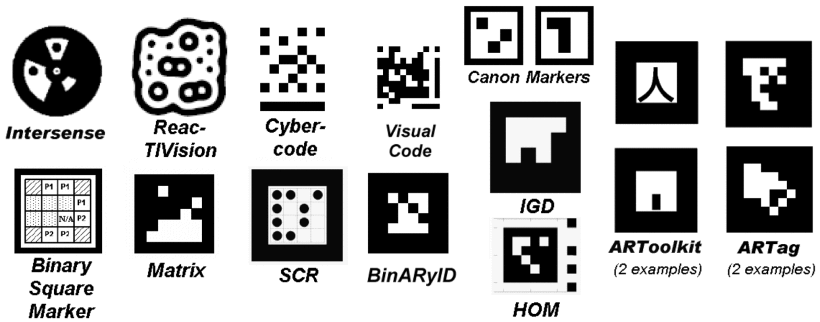
\includegraphics[width=0.9\linewidth,fbox]{figs/fiducial_marks.png}
    \caption{Exemplos de marcas fiduciais.}
    \source{\citeonline{fiala_designing_2010}.}
    \label{fiducial}
\end{figure}

Códigos de barra e QR Codes não são considerados marcas fiduciais. O objetivo destes é carregar informações e não tem dados suficientes para permitir a sua localização. Entretanto, o uso de padrões bitonais (geralmente preto e branco) dos QrCodes e códicos de barra é aproveitado nas marcas fiduciais, dado que isso facilita a detecção quando há variações de luminosidade.

TopCodes\footnote{\url{http://users.eecs.northwestern.edu/~mhorn/topcodes/}} é uma biblioteca de visão computacional projetada para permitir rápida detecção de marcas fiduciais. Além da identificação e da localização, a biblioteca informa o diâmetro e a orientação de cada marca. A biblioteca tem código aberto e é utilizada em diferentes projetos. \citeonline{hu_strawbies_2015} implementaram uma linguagem de blocos tangíveis para programar o personagem do ambiente Osmo ((\autoref{strawbies_topcodes}). \citeonline{viana_interface_2018} implementaram um ambiente de algoritmos sonoros para deficientes visuais, onde cada marca fiducial representou um instrumento musical (\autoref{bateria_topcodes}).

Uma desvantagem desse tipo de abordagem é o fato de o usuário encobrir as marcas durante a manipulação. A não detecção de uma peça pode prejudicar o desempenho de sistemas que precisam detectar objetos constantemente. Entretanto esse problema não é relatado nos trabalhos mencionados.

\begin{figure}[h!]
    \centering
    \begin{subfigure}{.4\textwidth}
        \centering
        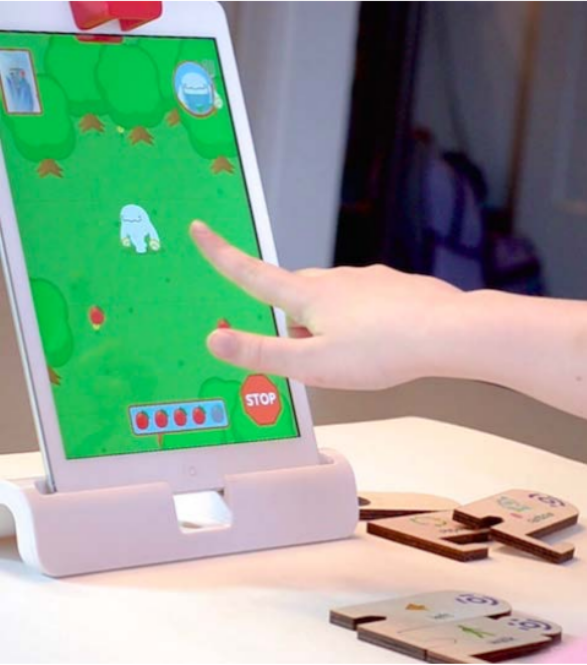
\includegraphics[width=.9\linewidth,fbox]{figs/topcodes_osmo.png}
        \caption{Tablet captura marcas fiduciais}
        \source{\citeonline{hu_strawbies_2015}.}
        \label{strawbies_topcodes}
    \end{subfigure}%
    \begin{subfigure}{.57\textwidth}
        \centering
        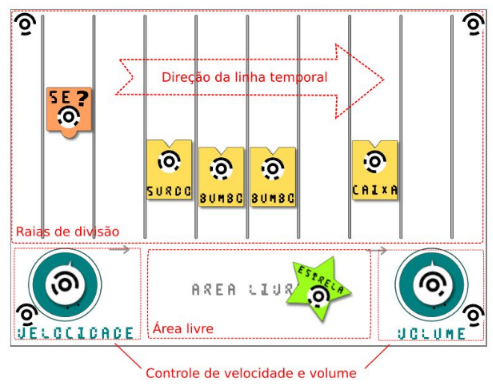
\includegraphics[width=.9\linewidth,fbox]{figs/topcodes_cassiano.png}
        \caption{Bateria de algoritmos sonoros tangível}
        \source{\citeonline{viana_interface_2018}.}
        \label{bateria_topcodes}
    \end{subfigure}
    \caption{Exemplos de uso da biblioteca TopCodes.}
    \label{topcodes_examples}
\end{figure}

\section{Realidade Aumentada}
\label{sec_realidade_aumentada}
A Realidade Aumentada (RA) é uma tecnologia que tem se popularizado nos últimos dez anos. Tem aplicações em inúmeros campos, entre os quais a medicina, a indústria, educação e entretenimento \cite{mekni_augmented_2014}. Apesar da popularização recente, as primeiras experiências com RA são atribuídas a Ivan Sutherland, que na década 1960 criou um dispositivo com pequenas telas próximas aos olhos, que permitiam ver o mundo real e adicionavam objetos virtuais adaptáveis às mudanças de perspectiva do usuário. Ainda hoje a RA se caracteriza por complementar a percepção do usuário ao associar elementos virtuais sobre elementos reais  \cite{parveau_3ivclass_2018}. Além da RA, existem outras técnicas que mostram elementos virtuais e proporcionam experiências realistas de interação, como a Realidade Virtual (RV). Essas técnicas se diferenciam pela quantidade de informação real ou virtual acessada.

Para melhor compreender essa associação \citeonline{milgram_augmented_1994} propõem o conceito de \textit{Virtual Continuum} (\autoref{fig_milgram}). Esse conceito tem de um lado a realidade, e do outro a virtualidade. A realidade obedece leis da natureza, como gravidade e velocidade. A virtualidade, por outro lado, pode ter suas próprias regras. Entre os dois opostos há um intervalo que mistura real e virtual, denominado Realidade Mista (RM). A RA se encontra à esquerda neste intervalo pois a maior parte da informação acessada pelo usuário existe no ambiente real, e apenas uma camada de objetos virtuais é adicionada. O conceito também apresenta a virtualidade aumentada, que seria a Realidade Virtual. Por ter a maior parte do conteúdo gerado pelo computador e apenas preservar alguns aspectos da realidade, a RV se encontra à direita no intervalo da Realidade Mista.

\begin{figure}[!htpb]
  \centering
  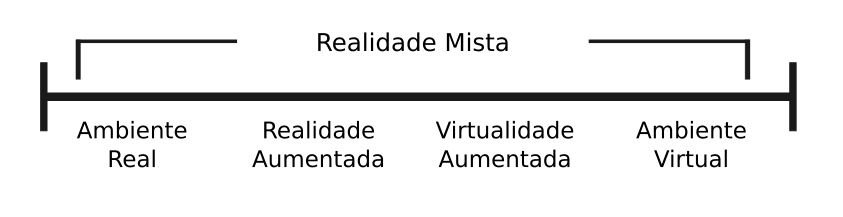
\includegraphics[width=.6\linewidth,fbox]{figs/milgram.png}
  \caption{\textit{Continuum} de realidade-virtualidade de Milgram (1994).}
  \source{Adaptado de \citeonline{milgram_augmented_1994}.}
  \label{fig_milgram}
\end{figure}

%Outra definição Na RV o usuário tem uma experiência realista de interação, porém todos os elementos que ele vê são gerados por computador, sem ter acesso ao mundo real. Essa experiência geralmente é alcançada com dispositivos como óculos e capacetes de visualização \cite{rodello_realidade_2010}. Na RA, ao contrário, o usuário acessa o mundo real e vê objetos virtuais associados a figuras reais que são identificadas por meio de visão computacional. Não há, entretanto, interação direta com os objetos virtuais a não ser movimentando as figuras às quais eles estão atrelados. Já na RM, a diferença é que o usuário pode interagir com os objetos virtuais, o que exige dispositivos especiais de visualização e identificação de gestos \footnote{Um exemplo de dispositivo com realidade mista é o HoloLens \url{https://www.microsoft.com/en-us/hololens}.}. 

\citeonline{azuma_recent_2001} acrescenta outros dois princípios além da combinação de objetos virtuais e reais. Primeiro, o sistema deve executar de forma iterativa e em tempo real, de modo que as mudanças ocorram instantaneamente. Qualquer modificação de perspectiva ou de posicionamento dos objetos reais deve ser imediatamente refletida nos objetos virtuais percebidos pelo usuário. O segundo princípio define que deve haver um alinhamento dos objetos virtuais com os reais, denominado de \textit{registro}. Ou seja, o posicionamento dos objetos virtuais precisa fazer sentido em relação ao mundo real.

\subsection{Tecnologias para Criar Realidade Aumentada}

Para ser viável, a RA depende de um conjunto de tecnologias para mostrar objetos virtuais e rastrear os objetos reais. A \autoref{subsub_displays} apresenta diferentes tipos de displays e a seção \autoref{subsub_tracking} cita tecnologias de rastreio/registro.

\subsubsection{Displays}
\label{subsub_displays}

Um dos objetivos da RA é produzir integrações de modo que o usuário não consiga distinguir o real do virtual. Para isso diferentes tipos de displays tem sido desenvolvidos. Os displays são responsáveis por dispor o objeto virtual em algum ponto entre a retina do observador e o ambiente real. Eles podem estar ou não acoplados ao observador, ser de uso individual ou permitir interações em grupo. Há três classes principais de dispositivos utilizados para mostrar os objetos virtuais: os \textit{head-worn displays}, os \textit{handheld displays} e \textit{projection displays} \cite{azuma_recent_2001}.

\begin{figure}[h]
    \centering
    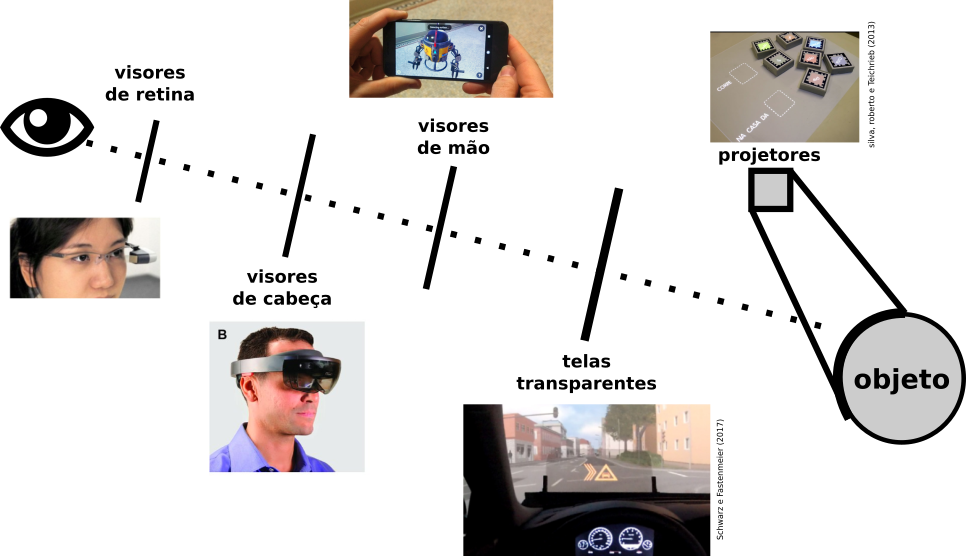
\includegraphics[width=.9\linewidth,fbox]{figs/ra_displays.png}
    \caption{Interseção de objetos virtuais entre o olho humano e o mundo real. }
    \source{Adaptado de Oliver e Raskar (2015).}
    \label{fig:ra_displays}
\end{figure}

\subsubsubsection*{Head-worn displays}

Os \textit{head-worn displays} (visores de cabeça) são usados na cabeça do usuário e mostram imagens em visores próximos aos olhos. Essa abordagem foi utilizada por Ivan Sutherland na primeira aplicação de RA. Esses visores são comumente de dois tipos. O primeiro tipo é um visor transparente, como uma lente de óculos, que permite ver o mundo real e ao mesmo tempo mostra os objetos virtuais. O segundo tipo são visores como telas de LCD. Nessa abordagem uma câmera capta o mundo real e transmite ao usuário por meio do visor, que adiciona os objetos virtuais na cena. \citeonline{azuma_recent_2001} ainda cita um terceiro tipo de display de cabeça que projeta as imagens diretamente na retina humana por meio de \textit{lasers} de baixa potência.

\subsubsubsection*{Handheld displays}

Os \textit{handheld displays} (visores de mão) representam o modo mais comum e acessível de RA. É o que \citeonline{milgram_augmented_1994} denomina \textit{window-on-the-world}, ou seja, uma janela no mundo. Os objetos virtuais aparecem em um visor de um dispositivo que o usuário segura com as mãos (um \textit{smartphone} ou \textit{tablet}), que pode ser comparado a uma lupa. Por meio dessa "janela" ou "lupa" o usuário visualiza o mundo real e os objetos virtuais. Por ser o mais comum, há um conjunto de projetos que visam facilitar o desenvolvimento de aplicações de AR para dispositivos móveis, como o ARCore\footnote{\url{https://developers.google.com/ar}}, da Google.

\subsubsubsection*{Projection Displays}

Os \textit{projection displays} (visores de projeção) projetam a informação virtual diretamente sobre o ambiente físico. No caso mais simples, utiliza-se um ou mais projetores fixos no ambiente. Outra estratégia, mais complexa, é utilizar projetores posicionados na cabeça do usuário, mas há a desvantagem do peso do equipamento \cite{azuma_recent_2001}. Ambos os casos precisam considerar as características da superfície de projeção, pois superfícies irregulares tendem a deformar a imagem projetada.

A projeção direta de objetos virtuais no ambiente físico se dá no campo da Realidade Aumentada Espacial. Quando usa projetores, \citeonline{resch_enhancing_2016} denomina como Realidade Aumentada Espacial Projetiva, aqui tratada simplesmente como RA Projetiva. Ele cita como vantagens dessa abordagem:
\begin{itemize}
    \item Não haver erros de profundidade em relação ao ambiente físico, pois os objetos virtuais são projetados diretamente no ambiente;
    \item Ausência de capacetes especiais ou dispositivos que precise segurar com as mãos, aumentando a segurança e liberando ações manuais;
    \item O desacoplamento espacial em relação ao usuário permite que os objetos virtuais sejam acessados por grupos maiores de usuários, o que não ocorre com capacetes ou smartphones;
    \item A resolução obtida com projeção tende a ser maior do que a oferecida por dispositivos acoplados à cabeça.
\end{itemize}

Entretanto há também desvantagens. Ambientes com iluminação forte tendem a ofuscar a imagem projetada, o que exige projetores mais potentes ou projetores a \textit{laser}. O segundo problema é a possibilidade de o usuário obstruir a projeção. Uma forma de mitigar esse problema é o uso de mais de um projetor de maneira sincronizada.

\begin{figure}[h]
    \centering
    \begin{subfigure}{.33\textwidth}
        \centering
        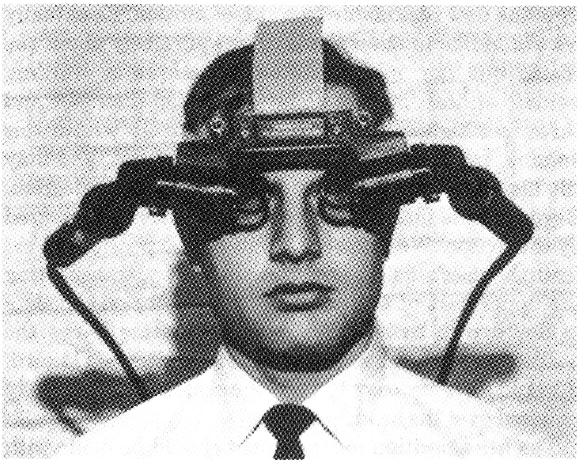
\includegraphics[width=.9\linewidth,fbox]{figs/ivan_sutherland_device.png}
        \caption{Visor de cabeça criado por Ivan Sutherland em 1968.}
        \label{fig_ivan_sutherland}
        \source{\citeonline{sutherland_head-mounted_1968}.}
    \end{subfigure}%
    \begin{subfigure}{.55\textwidth}
        \centering
        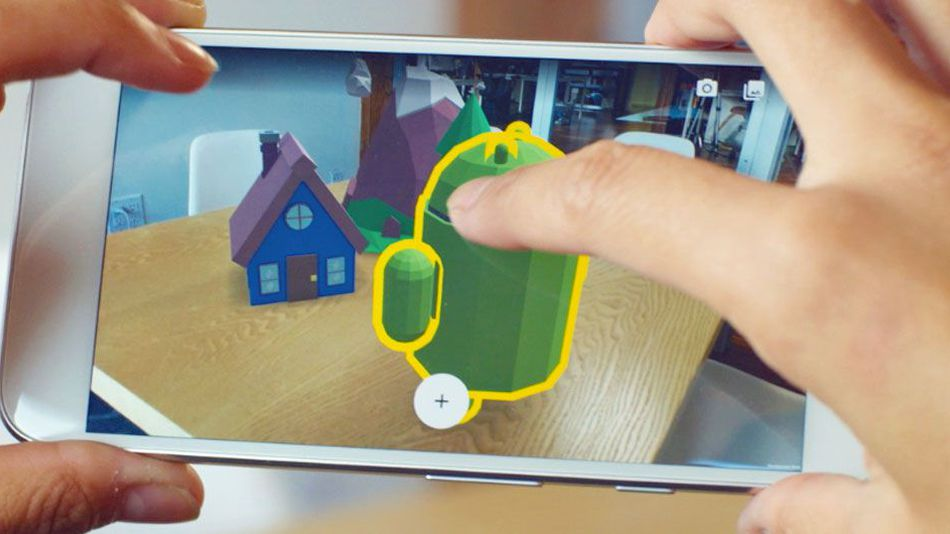
\includegraphics[width=.9\linewidth,fbox]{figs/arcore.jpg}
        \caption{Visor de mão, em aplicação para smartphone criada com ARCore.}
        \label{fig_arcore}
    \end{subfigure}%
    \caption{Dispositivos para criar realidade aumentada.}
    \label{fig_ra_devices}
\end{figure}

\subsubsection{Tecnologias de Rastreamento}
\label{subsub_tracking}
O rastreio preciso, rápido e robusto do observador, bem como dos objetos reais e virtuais é um aspecto crucial para criar aplicações de RA convincentes \cite{bimber_spatial_2005}. Um conjunto de métodos são utilizados para esse rastreamento, com base em sensores como giroscópios, acelerômetros e sensores magnéticos, mas a maior parte se baseia em captação de imagem \cite{resch_enhancing_2016}. As seguir são apresentadas brevemente duas técnicas de rastreamento com captação de imagem.

\subsubsubsection*{Marcas Fiduciais}

As abordagens de rastreamento com base em captação de imagem precisam extrair características presentes na cena observada. Essa características podem existir naturalmente ou serem implantadas artificialmente em pontos de interesse. As marcas implantadas artificialmente tem o benefício de serem reconhecidas com mais facilidade por algoritmos de visão computacional. As marcas fiduciais, apresentadas na \autoref{sub_sec_fiduciais}, além de serem utilizadas em aplicações com interfaces tangíveis, são amplamente aplicadas na RA. 

O processo de identificação das marcas artificiais inicia com a captura da imagem, à qual aplica-se um filtro para transformá-la em preto e branco. Segundo \citeonline{resch_enhancing_2016} essa etapa é complexa devido à variações de luminosidade do ambiente. Depois deste filtro, são extraídos os contornos das marcas e por fim o código binário de cores interno à cada marca é decodificado. 
No campo da RA projetiva, uma desvantagem do uso de marcas especiais é o fato da projeção alterar as características da marca, principalmente as cores, prejudicando sua identificação. Para evitar esse problema é necessário desativar a projeção enquanto a câmera capta as marcas, mas isso impede a projeção em tempo real \cite{resch_enhancing_2016}.

\subsubsubsection*{Características Naturais}
As características naturais são estruturas que pertencem à cena sem em si, ou seja, não há modificações artificiais para facilitar sua identificação. Essas características precisam, assim como as marcas fiduciais, ser identificáveis em condições de iluminação e posições diversas. Há dois tipos de rastreio naturais, os quais buscam identificar bordas e pontos.

A identificação de bordas foi um dos primeiros métodos de rastreio de características naturais utilizados, pela facilidade de identificação e robustez em condições variantes de iluminação. Nessa técnica, uma câmera capta um quadro da cena, que é comparado com um modelo 3D do objeto a ser identificado. Essa comparação tem como saída a estimativa da posição atual do objeto \cite{resch_enhancing_2016}. 

Por outro lado, a identificação de pontos é uma alternativa que também é robusta a variações de luminosidade. Pontos de interesse são previamente cadastrados em uma base de dados criada a partir de um modelo 3D observado de diferentes pontos de vista. Os mesmos pontos são, posteriormente, extraídos da imagem captada pela câmera, e comparados aos pontos armazenados. Essa busca permite então encontrar a posição atual aproximada do objeto real. 

\subsection{RA Projetiva}
\label{sub_aplicacoes_ra_projetiva}

A RA projetiva é um subtipo da Realidade Aumentada Espacial, a qual normalmente associa um ou mais projetores para produzir o conteúdo virtual e câmeras para captar os objetos reais. \citeonline{bimber_spatial_2005} comentam que os ambientes com uso de projeção se popularizaram na década de 1990. Um exemplo desta época é o CAVE, um quarto cujas paredes serviam de telas para criar uma experiência imersiva. Outros exemplos, com menos imersão, tem projeção em áreas menores, como mesas, paredes, paredes curvadas e esferas.

A RA projetiva tem encontrado aplicações em áreas diversas. Uma das abordagens é simular a visualização de estruturas internas à uma superfície, para facilitar o manuseio das mesmas sem a necessidade de abrir a superfície. Exemplos são órgãos humanos, no campo da medicina, e peças de veículos, na mecânica. Em um trabalho neste sentido, \citeonline{bornemann_exploration_2020} combinam três projetores apontados para um manequim e projetam os órgãos humanos permitindo estudar sua localização (\autoref{fig_bornemann}). Essa projeção se modifica conforme os movimentos da cabeça do observador, dando às estruturas projetadas um aspecto tridimensional. Essa técnica potencialmente facilitaria cirurgias não invasivas, nas quais atualmente o cirurgião divide a atenção entre o corpo do paciente e um monitor. A projeção dos órgãos sobre o corpo do paciente evitaria a divisão de atenção, mantendo os olhos direcionados para um único local.

Outra aplicação na área médica é o tratamento de pacientes com fobias de pequenos animais. \citeonline{wrzesien_treating_2015} usam um projetor para mostra os animais que o paciente teme e ele pode interagir com os mesmos de forma controlada (\autoref{fig_wrzesien}). No campo da indústria, \citeonline{sand_smartassembly_2016} desenvolveram o smARt.assembly, que é um sistema de assistência à trabalhadores responsáveis por montagens manuais. O sistema tem um projetor apontado para uma estante com peças, onde destaca a próxima peça a ser utilizada e também mostra como encaixá-la na produto a ser montado (\autoref{fig_sand}).

\begin{figure}
    \centering
    \begin{subfigure}{.33\textwidth}
        \centering
        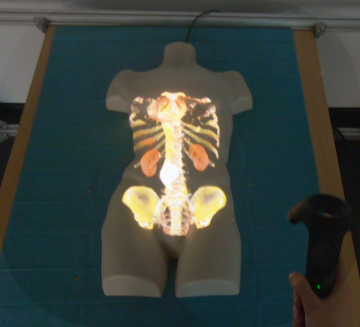
\includegraphics[width=.9\linewidth,fbox]{figs/bornemann.png}
        \caption{Projeção de órgãos internos.}
        \label{fig_bornemann}
        \source{\citeonline{bornemann_exploration_2020}.}
    \end{subfigure}%
    \begin{subfigure}{.33\textwidth}
        \centering
        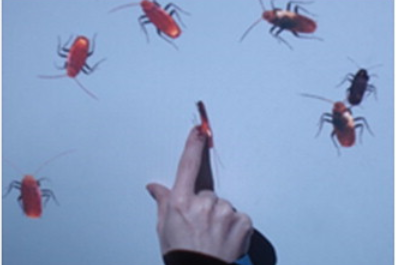
\includegraphics[width=.9\linewidth,fbox]{figs/wrzesien.png}
        \caption{Tratamento de fobias.}
        \label{fig_wrzesien}
        \source{\citeonline{wrzesien_treating_2015}.}
    \end{subfigure}%
    \begin{subfigure}{.33\textwidth}
        \centering
        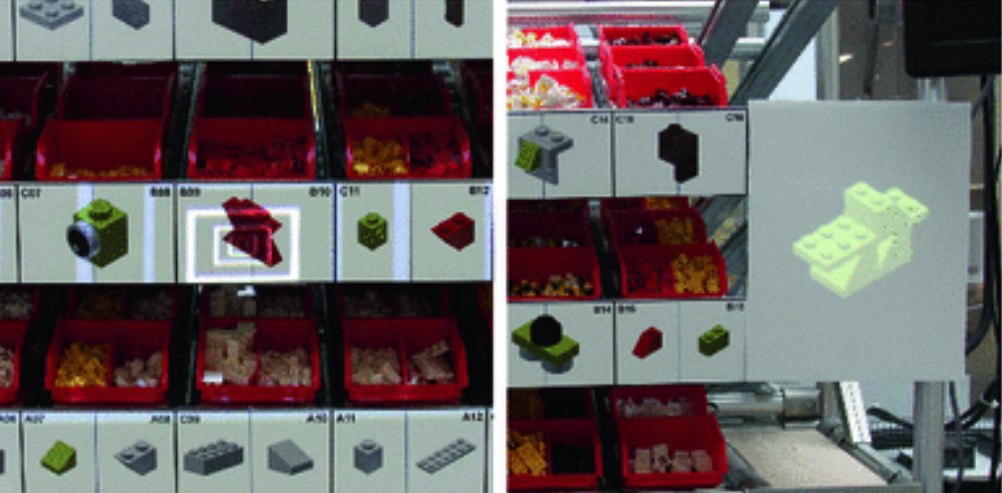
\includegraphics[width=.9\linewidth,fbox]{figs/sand.png}
        \caption{Auxílio em linhas de montagem.}
        \label{fig_sand}
        \source{\citeonline{sand_smartassembly_2016}.}
    \end{subfigure}%
    \caption{Aplicações de RA Projetiva.}
    \label{fig_proj_ra_applications}
\end{figure}

\subsubsection{RA Projetiva Aplicada a Ferramentas Educacionais}
\label{sub_sub_aplicacoes_ra_projetiva_educacao}

A \ac{RA} tem potencial educacional ao motivar os estudantes e promover a interação entre o conteúdo e o aluno \cite{silva_evaluating_2013}. Portanto, além das aplicações na medicina e na indústria, a RA projetiva também se aplica a ferramentas educacionais. Além da RA projetiva, essas ferramentas normalmente utilizam elementos tangíveis que servem como entradas para sistemas câmera-projetor. Câmeras captam os elementos tangíveis e algoritmos de visão computacional identificam esses elementos analisando suas marcas especiais ou suas características naturais. Como saída, um projetor emite os elementos virtuais.

A vantagem de unir a RA projetiva com interfaces tangíveis em aplicações educacionais está no favorecimento das interações em grupo. Sabe-se que as interações sociais favorecem o aprendizado por meio do \textit{scaffolding} (\autoref{sub_jerome_bruner}). A combinação \textit{RA projetiva-interfaces tangíveis} favorece interações em grupo de dois modos. Por um lado, a RA projetiva mostra os objetos virtuais a mais de um usuário ao mesmo tempo. Por outro lado, as interfaces tangíveis permitem a manipulação de objetos físicos por mais de um usuário simultaneamente \cite{burleson_active_2018, horn_tangible_2012}.

\begin{figure}[h]
    \centering
    \begin{subfigure}{.49\textwidth}
        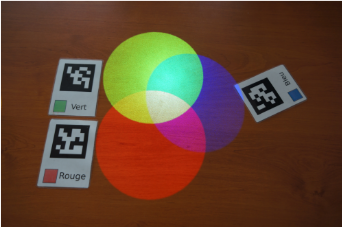
\includegraphics[width=.9\linewidth,fbox]{figs/nectar.png}
        \caption{Nectar - Exploração de modos de cores.}
        \label{fig_nectar}
        \source{\citeonline{laviole_nectar_2018}.}
    \end{subfigure}
    \begin{subfigure}{.49\textwidth}
        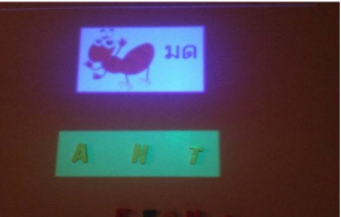
\includegraphics[width=.9\linewidth,fbox]{figs/pinkaew.png}
        \caption{Tangible Word Game - Alfabetização.}
        \source{\citeonline{pinkaew_interactive_2014}.}
        \label{fig_pinkaew}
    \end{subfigure}
    \begin{subfigure}{.49\textwidth}
        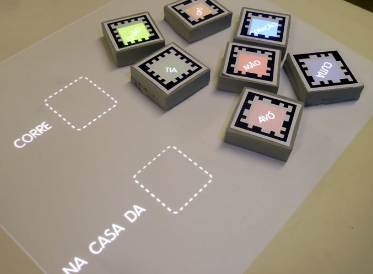
\includegraphics[width=.9\linewidth,fbox]{figs/roberto.png}
        \caption{ARBlocks - Atividade de alfabetização.}
        \label{fig_silva_roberto_ra}
        \source{\citeonline{silva_evaluating_2013}.}
    \end{subfigure}
    \begin{subfigure}{.49\textwidth}
        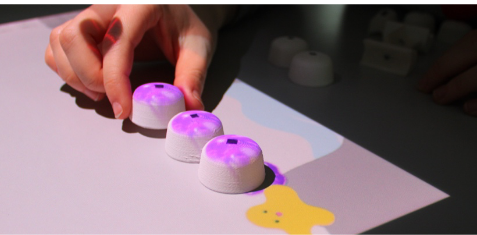
\includegraphics[width=.9\linewidth,fbox]{figs/mart.png}
        \caption{MaR-T - Atividade de matemática.}
        \label{fig_math}
        \source{\citeonline{besevli_mar_t_2019}.}
    \end{subfigure}
    \caption{Ferramentas educacionais usando RA projetiva.}
\end{figure}

\citeonline{laviole_nectar_2018} apresenta uma ferramenta para exploração de modelos de cores aditivas e subtrativas (\autoref{fig_nectar}). A soma das cores primárias no modo aditivo (verde, vermelho e azul) resulta em branco, e a soma das cores primárias no modo subtrativo (ciano, magenta e amarelo) resulta em preto. Na ferramenta de Laviole, cartas com marcas fiduciais representam as cores, e ao lado de cada carta é projetado um círculo colorido que pode ser sobreposto à outros círculos. Além disso, há uma carta que permite trocar entre o modo aditivo e subtrativo. Um questionário guia os estudantes na exploração das cartas, com perguntas como: o que é a cor branca? o que você vê ao combinar vermelho, verde e azul? Tentando responder as perguntas, os estudantes exploram as combinações de modo ativo e colaborativo, possivelmente compreendendo esse fenômeno físico complexo.

Outras duas ferramentas visam promover a alfabetização. \citeonline{pinkaew_interactive_2014} identificam sequências de letras de plástico e projetam figuras referentes às palavras formadas. Uma câmera de infravermelho capta as letras, técnica que apresentou problemas de diferenciação de letras similares como Q, O, e C, devido à fontes de luz inadequadas. Na segunda ferramenta \citeonline{silva_evaluating_2013} avaliam o ARBlocks, desenvolvido por \citeonline{roberto_dynamic_2013}. O ARBlocks, apresentado na \autoref{sub_arblocks}, possui blocos tangíveis customizáveis via projeção de conteúdo virtual, bem como feedbacks luminosos e sonoros. A atividade proposta consistiu na formação de rimas ao completar frases com blocos tangíveis (\autoref{fig_silva_roberto_ra}). A avaliação com grupo de teste e de controle concluiu que o grupo de teste, que tinha dificuldade de aprendizado, conseguiu obter aprendizados semelhantes ao grupo de controle nos assuntos que foram abordados usando RA. A professora da turma também mencionou motivação e engajamento das crianças no uso da ferramenta, a qual afirma tê-las incentivado a lerem mais.

A última ferramenta de exemplo aborda o conteúdo de matemática com o objetivo de auxiliar crianças de 3 a 5 anos no desenvolvimento da representação numérica não-simbólica, ou seja, a comparação entre grandezas (tamanhos, quantidades) antes do reconhecimento dos símbolos numéricos. Denominada MaR-T, a ferramenta desenvolvida por \citeonline{besevli_mar_t_2019} mostra uma sequência de atividades nas quais a criança agrupa pedrinhas de modo a permitir a passagem de um personagem virtual sobre buracos e rios. As pedras são empilhadas, na horizontal ou agrupadas para a criança compreender a conservação de quantidades em diferentes disposições. Em cada etapa, a criança coloca a mão sobre o grupo que possui mais ou menos peças. Em termos de hardware e software, a aplicação utiliza um projetor acoplado a um \textit{smartphone} Android, e as peças utilizam adesivos refletores que facilitam a identificação por meio da biblioteca OpenCV.

\subsubsection{Métodos de Entrada}
Os métodos de entrada desses sistemas são diversos. No caso do smaArt.assembly o trabalhador controla o sistema por meio de pedais, para não perder tempo de trabalho manual. Já o sistema de \citeonline{bornemann_exploration_2020} combina a captação de movimentos da cabeça do usuário por meio de controles remotos que tem sua posição rastreada por sistemas específicos. Ambos os trabalhos citam o reconhecimento de gestos como um método de entrada alternativo a ser testado futuramente. Já o trabalho de \citeonline{wrzesien_treating_2015} reconhece gestos captados por uma câmera, de modo que o paciente pode interagir com os animais projetados colocando a mão sobre eles. Métodos de entrada tradicionais também são aplicados. Plecher et al (2020) usam RA projetiva em uma exposição de museu, na qual os usuários interagem por meio de um \textit{tablet} para pintar uma estátua em exposição, de modo que as cores selecionadas no aparelho se refletem na escultura por meio de um projetor. Por fim, as ferramentas educacionais apresentadas (\autoref{sub_sub_aplicacoes_ra_projetiva_educacao}) tem em comum o uso de interfaces tangíveis com ou sem marcas fiduciais, que são identificadas por meio de câmeras.

\section{Considerações}

Este capítulo abordou temas fundamentais para guiar a criação de interfaces de programação para crianças. Olhar para o indivíduo que usará uma ferramenta, pensando no seu desenvolvimento cognitivo, limitações motoras e aspectos emocionais é a direção apontada Montessori, Piaget, Bruner e Papert. 

A segunda seção (\autoref{fundamentacao_pc}) abordou a definição de \acl{PC}. Apesar da falta de uma definição estabelecida, percebe-se que há grande relação com programação, mas que também vai além dela. Os pilares decomposição, reconhecimento de padrões e abstração podem ser aplicados em resolução de problemas por vezes sem o uso de dispositivos computacionais. A depuração, por estar associada à tarefa de programar, por vezes tem importância secundária e não é mencionada em definições do PC. 

A seguir foram abordadas duas classificações de brinquedos programáveis e diferentes alternativas tecnológicas empregadas em suas interfaces. Percebe-se que autores incentivam o uso de interfaces tangíveis para crianças, e que a programação em blocos é a metáfora mais utilizada para representar comandos. Percebe-se a preocupação com o design dos blocos, que ao evitar o uso de letras considera se o público é ou não alfabetizado.

Um último item abordado foram novas formas e interação: interfaces de realidade virtual, aumentada e mista. Como demonstrado no próximo capítulo, poucos brinquedos programáveis utilizam esse tipo de interface, e portanto investigar a adequação dessas tecnologias para o público infantil é um tema a ser explorado.

% \begin{table}[!htbp]
% \begin{center}
% \begin{footnotesize}
% \caption{Exemplo de Tabela: Extração e Análise dos Dados - RSL 02}
% \label{t_apendiceC-rsl}

% \begin{tabular}{l|c|c|c|c|c|c|}
% \cline{2-7}
%  & \textbf{ACM} & \textbf{IEEExplore} & \multicolumn{1}{l|}{\textbf{ScienceDirect}} & \textbf{Scopus} & \textbf{Springer} & \textbf{Total de artigos} \\ \hline
% \multicolumn{1}{|l|}{\textbf{Resultado da \textit{string} de busca}} & 24 & 26 & 9 & 49 & 154 & 262 \\ \hline
% \multicolumn{1}{|l|}{\textbf{Trabalhos repetidos}} & 7 & 1 & 7 & 22 & 0 & 37 \\ \hline
% \multicolumn{1}{|l|}{\textbf{Trabalhos removidos}} & 15 & 20 & 2 & 21 & 153 & 211 \\ \hline
% \multicolumn{1}{|l|}{\textbf{Trabalhos pré-selecionados}} & 2 & 5 & 0 & 6 & 1 & 14 \\ \hline
% \multicolumn{1}{|l|}{\textbf{Trabalhos aceitos}} & 1 & 1 & 0 & 2 & 0 & 4 \\ \hline
% \end{tabular}

% \end{footnotesize}
% \end{center}
% \raggedright Fonte: Elaborada pelo próprio autor.
% \end{table}
